\section{Implementation}\label{sec:implementation}

%In this section the suggested a structure in section \ref{sec:Structure} implemented with the numerical solutions in section \ref{se:preissmann_scheme}-\ref{sec:concentrate}, is tested and verified.
In this section, the implementation of the various parts, which the simulation environment consist of, is explained. The chosen structure, which is described in section \ref{sec:Structure}, is seen in figure \ref{fig:Basic_implementation}. 

\begin{figure}[H]
\centering
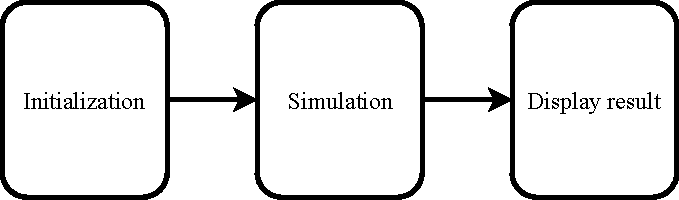
\includegraphics[width=0.75 \textwidth]{report/simulation/pictures/Basic_implementation.pdf}
\caption{Chosen structure of simulation environment.}
\label{fig:Basic_implementation}
\end{figure}

The first part to be elaborated upon is the initialization.

 \subsection*{Initialization}

For the setup procedure of the simulation in list form, the specifications part, shown in figure \ref{fig:sys_setup}, needs to be defined. The necessary parameters in the list for both pipe and tank can be seen in table \ref{tab:init_list}. 
\begin{table}[H]
\begin{enumerate} 
	\item Pipe
	\begin{itemize}
		\item Length [m]
		\item Sections (Number of sections the pipe should be split in to)
		\item $\text{S}_\text{b}$ (Slope) [\textperthousand]
		\item $\Delta$x = Length/Sections [m]
		\item Diameter [meter]
		\item Theta (parameter used in Preissmann scheme)
		\item $\text{Q}_{\text{f}}$ (maximum flow found by Manning formula, see equation \ref{eq:qf_for_flow}) [$\text{m}^\text{3}/\text{s}$]
		\item Side/lateral inflow present 
		\item Section location in data 
	\end{itemize}
	\item Tank
	\begin{itemize}
		\item Size [$\text{m}^\text{3}$]
		\item Height [m]
		\item Area = Size / Height [$\text{m}^\text{2}$]
		\item Maximum outflow [$\text{m}^\text{3}/\text{s}$]
		\item Section location in data 
	\end{itemize}
	
\end{enumerate}
\caption{List of parameters for pipe and tank.}
\label{tab:init_list}
\end{table}
Some parameters can be found from others and are set to be calculated automatically. 
%Furthermore an item is added that indicates in which section of the obtained simulation data the specific output of the component is located. This item is given the number of the order in which the component appears in the list. 
Furthermore, an item is added to the list which indicates, where the initial and simulated data, for the specific item can be found.
To give an overview of the system to be simulated, and to easily be able to locate specific parameters needed during simulation, three structures are returned to the workspace. These are named ``pipe\_spec'', ``tank\_spec'' and ``sys\_setup''. The first two structures holds the information shown in table \ref{tab:init_list} respectively. The last one, ``sys\_setup'', holds information about the various parts indexed in the order the system is set up and simulated. In figure \ref{fig:sys_setup_matlab} the content of ``sys\_setup'' is shown for a setup with two pipes and a tank.

\begin{figure}[H]
\centering
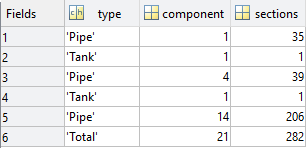
\includegraphics[width=0.5 \textwidth]{report/simulation/pictures/sys_setup_matlab.png}
\caption{Display of structure showing system setup information in MATLAB.}
\label{fig:sys_setup_matlab}
\end{figure}

An initialization scheme is constructed as per figure \ref{fig:simple_sewer} where adjoining pipes are considered as one part of the system and each tank is an individual part, which means that tanks are used as a separator between parts consisting of pipes.
The iterative scheme is shown in figure \ref{fig:preissmann_grid_scheme_exampel} requires that boundary conditions are found before the iterative Preissmann scheme can be started. It has been decided by the project group that input should be given in flow, as input in height would be needed to be specific for the pipe inserted, to make the simulation universal. This means that from an initial input flow the corresponding height in the pipes needs to be found. By equation \ref{eq:calc_for_flowv2} flow can be obtained from height, but that equation is transcendental, as it can not be solved analytically for height. This means that other means are necessary to obtain height from a flow. Various iterative schemes exist to solve such equations, but due to the desire to keep computation time at a minimum, use of such schemes is refrained from.
A solution to the problem is that for each pipe, during initialization, a data set from zero to the diameter of the pipe in sufficient steps is created, and from which the corresponding flow is obtained by equation \ref{eq:calc_for_flowv2}. From this data, a curve fitted polynomial can be obtained by the MATLAB curve fitting toolbox or a lookup table can be constructed. Flow data is generated for 10.000 height steps for a pipe with the parameters shown in table \ref{tab:pipe_figure_parameters}.

\begin{table}[H]
\centering
\begin{tabular}{|c|l|} \hline
Diameter & 0,9 meter \\ \hline
Slope ($\text{I}_\text{b}$) & 3 \textperthousand \\ \hline 
Length & 200 meter \\ \hline
Sections & 10 \\ \hline
 \end{tabular} 
\caption{List of parameters used to obtain data shown in figure \ref{fig:curvefit_comparision}}
\label{tab:pipe_figure_parameters}
 \end{table}

In figure \ref{fig:curvefit_comparision} a comparison is shown of the generated data and a ninth order polynomial fitted to the data.

\begin{figure}[H]
 \centering
 % This file was created by matlab2tikz.
%
%The latest updates can be retrieved from
%  http://www.mathworks.com/matlabcentral/fileexchange/22022-matlab2tikz-matlab2tikz
%where you can also make suggestions and rate matlab2tikz.
%
\definecolor{mycolor1}{rgb}{0.00000,0.44700,0.74100}%
%
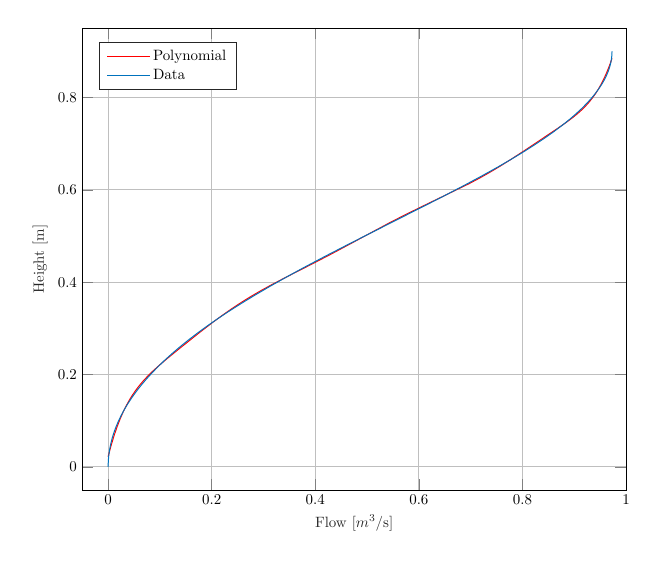
\begin{tikzpicture}[thick,scale=0.9, every node/.style={scale=0.6}]

\begin{axis}[%
width=3.021in,
height=2.566in,
at={(0.758in,0.481in)},
scale only axis,
xmin=-0.05,
xmax=1,
xlabel style={font=\color{white!15!black}},
xlabel={Flow [$\text{m}^\text{3}$/s]},
ymin=-0.05,
ymax=0.95,
ylabel style={font=\color{white!15!black}},
ylabel={Height [m]},
axis background/.style={fill=white},
xmajorgrids,
ymajorgrids,
legend style={at={(0.03,0.97)}, anchor=north west, legend cell align=left, align=left, draw=white!15!black}
]
\addplot [color=red]
  table[row sep=crcr]{%
0	0.0222641876397454\\
0.00583788013141662	0.0468505124572859\\
0.0116757602628333	0.0685037472280541\\
0.01751364039425	0.0875962984430564\\
0.0233515205256666	0.104462594043742\\
0.0291894006570832	0.119402060847026\\
0.0350272807884998	0.132681928352076\\
0.0408651609199165	0.14453986606579\\
0.0467030410513332	0.155186461298207\\
0.0535139012046525	0.166323129330026\\
0.0603247613579719	0.176319581381477\\
0.0681086015331941	0.186627394570619\\
0.0768654217303191	0.1971234679247\\
0.0865952219493469	0.207784706738995\\
0.0982709822121801	0.219634930070442\\
0.113838662562624	0.23449066785112\\
0.138163163110194	0.256755738358134\\
0.176109383964402	0.290671244351543\\
0.201406864533874	0.312526360051635\\
0.221839444993832	0.329374050052282\\
0.240326065409985	0.34381856012056\\
0.257839705804235	0.35673446219757\\
0.275353346198485	0.368905237211488\\
0.293839966614638	0.381009693497422\\
0.314272547074596	0.393647570538794\\
0.339570027644068	0.408528726872221\\
0.390164988783012	0.437347221406009\\
0.429084189659123	0.459928516339826\\
0.468003390535234	0.483262809711989\\
0.54389583224365	0.528968698128539\\
0.574058212922636	0.546263994393304\\
0.604220593601622	0.562860267064146\\
0.696653695682386	0.613119065583713\\
0.717086276142344	0.62530025086964\\
0.736545876580399	0.637586486102553\\
0.756005477018455	0.650574852430809\\
0.777411037500316	0.665605335087019\\
0.803681498091691	0.684833203666043\\
0.864979239471565	0.730734878672607\\
0.884438839909621	0.745858014555948\\
0.897087580194357	0.756440925031475\\
0.906817380413385	0.765353228191959\\
0.914601220588607	0.773208230042211\\
0.922385060763829	0.781942336734848\\
0.929195920917148	0.790515086732738\\
0.935033801048565	0.798722858348917\\
0.940871681179982	0.807888165233192\\
0.946709561311398	0.818188953039921\\
0.952547441442815	0.829827057099856\\
0.958385321574232	0.8430304635012\\
0.963250221683745	0.855413188684596\\
0.968115121793259	0.869225396536382\\
0.972980021902773	0.884648045759077\\
};
\addlegendentry{Polynomial}

\addplot [color=mycolor1]
  table[row sep=crcr]{%
0	0\\
0.00030642296001504	0.01233\\
0.00122592449248948	0.02466\\
0.00275919619829157	0.03699\\
0.00492531381189298	0.04941\\
0.00771691837291222	0.0618300000000001\\
0.0111359602571995	0.07425\\
0.0152163500161991	0.0867600000000001\\
0.0199744759873318	0.09936\\
0.02542711466865	0.11205\\
0.0315913434853029	0.12483\\
0.0384338333138317	0.13761\\
0.0460682367603654	0.15057\\
0.0544660114484651	0.16362\\
0.0637094855914684	0.17685\\
0.0738302832003164	0.19026\\
0.0847840346449592	0.20376\\
0.0967472281174419	0.21753\\
0.109678802055319	0.23148\\
0.123697951078652	0.2457\\
0.138846482140551	0.26019\\
0.155163670747372	0.27495\\
0.172793050923732	0.29007\\
0.191782482726017	0.30555\\
0.212292745916907	0.32148\\
0.234499027859045	0.33795\\
0.25845887409398	0.35496\\
0.284486130286045	0.37269\\
0.312918691318617	0.39132\\
0.344254168236911	0.41112\\
0.37915911064623	0.43245\\
0.419079139891965	0.45612\\
0.466907719593891	0.48375\\
0.53413117460992	0.52182\\
0.638838688603708	0.58113\\
0.684244287950606	0.60759\\
0.720760960442891	0.62955\\
0.751794914662872	0.6489\\
0.778966712722586	0.66654\\
0.802970121524758	0.68283\\
0.824328787062596	0.69804\\
0.843524532554507	0.71244\\
0.860764663768599	0.72612\\
0.87624717181071	0.73917\\
0.890156294853092	0.75168\\
0.902569357193314	0.76365\\
0.913654569164784	0.77517\\
0.923559217305502	0.78633\\
0.93233869141443	0.79713\\
0.94005219868443	0.80757\\
0.946818481487701	0.81774\\
0.952682361805689	0.82764\\
0.957734233356883	0.83736\\
0.962003234496279	0.8469\\
0.9655201136824	0.85626\\
0.968316966985129	0.86544\\
0.97044491415244	0.87453\\
0.971919271555091	0.88353\\
0.972756442059394	0.89244\\
0.972980021902773	0.9\\
};
\addlegendentry{Data}

\end{axis}
\end{tikzpicture}%
\caption{Comparison between data obtained by equation \ref{eq:calc_for_flowv2} and the same data curve fitted to a ninth order polynomial.}
\label{fig:curvefit_comparision}
\end{figure}
The two plots in the figure are seemingly identical, but if observed closer the curve fit has what could be described as a low frequency oscillation compared to the plotted data. Furthermore, the curve fit does not reach the same endpoints. This will result in the height at the endpoints never to be zero or the diameter of the pipe when no inflow or maximum inflow is present. In figure \ref{fig:curvefit_comparision_split} the plot is separated into three for an easier overview.


\begin{figure}[H]
 \centering
 % This file was created by matlab2tikz.
%
%The latest updates can be retrieved from
%  http://www.mathworks.com/matlabcentral/fileexchange/22022-matlab2tikz-matlab2tikz
%where you can also make suggestions and rate matlab2tikz.
%
\definecolor{mycolor1}{rgb}{0.00000,0.44700,0.74100}%
%
\begin{tikzpicture}

\begin{axis}[%
width=1.268in,
height=3.175in,
at={(2.2in,1.103in)},
scale only axis,s
xmin=-0.05,
xmax=0.255,
xlabel style={font=\color{white!15!black}},
xlabel={Flow [$\text{m}^\text{3}$/s]},
ymin=-0.05,
ymax=0.4,
ylabel style={font=\color{white!15!black}},
ylabel={Height [m]},
axis background/.style={fill=white},
xmajorgrids,
ymajorgrids,
legend style={at={(0.03,0.97)}, anchor=north west, legend cell align=left, align=left, draw=white!15!black}
]
\addplot [color=red]
  table[row sep=crcr]{%
0	0.0222641876397452\\
0.002	0.0310423507186317\\
0.004	0.0394452957735427\\
0.00600000000000001	0.0474896123161433\\
0.00800000000000001	0.0551913093444532\\
0.01	0.0625658308096022\\
0.012	0.0696280707783006\\
0.014	0.076392388295221\\
0.016	0.0828726219494472\\
0.018	0.0890821041491136\\
0.02	0.0950336751083192\\
0.022	0.100739696550368\\
0.024	0.106212065131344\\
0.026	0.111462225588011\\
0.028	0.11650118361396\\
0.03	0.121339518467939\\
0.032	0.125987395318202\\
0.034	0.130454577326758\\
0.036	0.134750437477274\\
0.038	0.138883970150443\\
0.04	0.142863802450524\\
0.042	0.146698205286753\\
0.044	0.150395104213308\\
0.046	0.153962090031438\\
0.048	0.15740642915736\\
0.05	0.16073507375949\\
0.052	0.163954671668528\\
0.054	0.167071576063904\\
0.056	0.170091854940031\\
0.058	0.17302130035581\\
0.06	0.175865437470771\\
0.062	0.178629533371213\\
0.064	0.181318605689683\\
0.066	0.183937431021079\\
0.068	0.186490553138647\\
0.07	0.188982291013104\\
0.072	0.191416746638089\\
0.075	0.194969485627572\\
0.078	0.198414344321734\\
0.081	0.201762648867287\\
0.084	0.20502481071003\\
0.087	0.208210377368781\\
0.09	0.211328081265009\\
0.093	0.214385886658126\\
0.097	0.218382201981612\\
0.101	0.222300129592964\\
0.105	0.226152997837096\\
0.11	0.230894979828061\\
0.116	0.236501118023782\\
0.123	0.24295746024834\\
0.131	0.250261133339763\\
0.141	0.259319049720577\\
0.153	0.270116802578941\\
0.164	0.279948128414307\\
0.173	0.287930045688142\\
0.181	0.294962503821962\\
0.188	0.301055217728628\\
0.195	0.307080190139537\\
0.201	0.312182600461743\\
0.207	0.317221300531533\\
0.213	0.322190515539783\\
0.219	0.327085077941444\\
0.224	0.331103612243363\\
0.229	0.33506502224299\\
0.234	0.338967534353605\\
0.239	0.342809785047988\\
0.244	0.346590827426471\\
0.249	0.35031013183293\\
0.254	0.353967581129179\\
0.256	0.35541329220446\\
};
\addlegendentry{Curve fit}

\addplot [color=mycolor1]
  table[row sep=crcr]{%
0	0\\
2.48304185804238e-05	0.00351000000000001\\
9.93232085852447e-05	0.00702000000000003\\
0.000223482969415489	0.01053\\
0.000397317355443627	0.01404\\
0.000620837059076784	0.01755\\
0.000894055787063641	0.02106\\
0.00122592449248948	0.02466\\
0.00161011236359732	0.02826\\
0.00204664383847447	0.03186\\
0.0025355465084787	0.03546\\
0.00307685105291455	0.03906\\
0.00367059116604707	0.04266\\
0.0043168034765097	0.04626\\
0.00501552745916467	0.04986\\
0.00576680533948298	0.05346\\
0.00657068199051475	0.05706\\
0.00742720482252818	0.06066\\
0.00833642366539827	0.06426\\
0.00929839064383481	0.06786\\
0.0103131600455422	0.07146\\
0.0113807881824109	0.07506\\
0.0125013332448436	0.07866\\
0.0136748551493265	0.08226\\
0.0149014153793596	0.08586\\
0.0161810768198663	0.08946\\
0.0175139035852057	0.09306\\
0.0188999608409186	0.09666\\
0.0203393146193402	0.10026\\
0.0218700338511926	0.10395\\
0.0234568901890829	0.10764\\
0.0250999562933016	0.11133\\
0.0267993048905982	0.11502\\
0.0285550085329623	0.11871\\
0.0303671393503522	0.1224\\
0.0322357687975712	0.12609\\
0.0341609673954891	0.12978\\
0.0361428044668208	0.13347\\
0.0381813478666689	0.13716\\
0.0403284787506254	0.14094\\
0.042535254094141	0.14472\\
0.0448017402173691	0.1485\\
0.0471280005690068	0.15228\\
0.0495140953962901	0.15606\\
0.0519600814105286	0.15984\\
0.0544660114484651	0.16362\\
0.0570319341297459	0.1674\\
0.0597211484251551	0.17127\\
0.0624733342640793	0.17514\\
0.0652885277920768	0.17901\\
0.06816675896115	0.18288\\
0.0711080511274374	0.18675\\
0.0741124206465261	0.19062\\
0.0772519632947214	0.19458\\
0.0804575616887742	0.19854\\
0.0837292079118647	0.2025\\
0.0870668845587141	0.20646\\
0.0904705642744617	0.21042\\
0.093940209293403	0.21438\\
0.0975568902819463	0.21843\\
0.101242453855357	0.22248\\
0.104996822806891	0.22653\\
0.108819906506757	0.23058\\
0.112798860871919	0.23472\\
0.116849381300941	0.23886\\
0.120971324178149	0.243\\
0.125164529004631	0.24714\\
0.129522307794482	0.25137\\
0.133954085548652	0.2556\\
0.138459632885561	0.25983\\
0.143038699635108	0.26406\\
0.147790793375852	0.26838\\
0.152618972114771	0.2727\\
0.157522898470217	0.27702\\
0.162606744485203	0.28143\\
0.16776873600719	0.28584\\
0.173008431171206	0.29025\\
0.178434668332884	0.29475\\
0.183940789913321	0.29925\\
0.189526230350682	0.30375\\
0.195304472276872	0.30834\\
0.201163941357038	0.31293\\
0.207221197384301	0.31761\\
0.213361364393635	0.32229\\
0.2197040632307	0.32706\\
0.226131092492676	0.33183\\
0.23276510614099	0.33669\\
0.239484561913134	0.34155\\
0.246415106055723	0.3465\\
0.253560216377759	0.35154\\
0.255102805548652	0.35262\\
};
\addlegendentry{Raw data}

\end{axis}

\begin{axis}[%
width=1.268in,
height=3.175in,
at={(4.216in,1.103in)},
scale only axis,
xmin=0.25,
xmax=0.75,
xlabel style={font=\color{white!15!black}},
xlabel={Flow [$\text{m}^\text{3}$/s]},
ymin=0.3,
ymax=0.7,
ylabel style={font=\color{white!15!black}},
%ylabel={y},
axis background/.style={fill=white},
xmajorgrids,
ymajorgrids,
legend style={at={(0.03,0.97)}, anchor=north west, legend cell align=left, align=left, draw=white!15!black}
]
\addplot [color=red]
  table[row sep=crcr]{%
0.249	0.35031013183293\\
0.255	0.354691666581612\\
0.262	0.359691701230937\\
0.269	0.364573586617454\\
0.276	0.369340965039136\\
0.283	0.373998737951873\\
0.29	0.378552926883383\\
0.297	0.383010521588671\\
0.305	0.387996670089977\\
0.313	0.392879507167007\\
0.322	0.398265932720645\\
0.332	0.404141450374147\\
0.343	0.410502990594094\\
0.357	0.418499578118555\\
0.401	0.443559700309453\\
0.415	0.451667310051688\\
0.428	0.459288735165773\\
0.442	0.467597762950332\\
0.457	0.476603835082106\\
0.476	0.488120525887873\\
0.515	0.511793040483264\\
0.529	0.520176602179741\\
0.541	0.527271293048054\\
0.552	0.533686029865968\\
0.563	0.540007271687931\\
0.574	0.546231314734744\\
0.585	0.552359493128402\\
0.597	0.558943399249206\\
0.61	0.56597490588983\\
0.626	0.574529055842827\\
0.658	0.59160882368966\\
0.67	0.59812620199676\\
0.68	0.603653211457091\\
0.689	0.608723309841312\\
0.697	0.613319949398277\\
0.705	0.618011892679499\\
0.713	0.622807955472417\\
0.72	0.627095546670148\\
0.727	0.631471829860599\\
0.734	0.635939028034652\\
0.741	0.64049797219494\\
0.748	0.645148024720358\\
0.751	0.647168315462028\\
};
\addlegendentry{Curve fit}

\addplot [color=mycolor1]
  table[row sep=crcr]{%
0.249976576240672	0.34902\\
0.259236020098798	0.3555\\
0.268770604516453	0.36207\\
0.278582982727352	0.36873\\
0.288810967283916	0.37557\\
0.299324710559653	0.3825\\
0.310264902062615	0.38961\\
0.321496592023219	0.39681\\
0.333162969488798	0.40419\\
0.345413837726718	0.41184\\
0.358111484464603	0.41967\\
0.371406904414949	0.42777\\
0.385306199342518	0.43614\\
0.399965417403482	0.44487\\
0.415544526316372	0.45405\\
0.432206111207128	0.46377\\
0.450269978113671	0.47421\\
0.470216918454365	0.48564\\
0.493006156351848	0.4986\\
0.521512531670953	0.51471\\
0.610182365254768	0.56475\\
0.631784954161493	0.57708\\
0.650385062883746	0.58779\\
0.667102191938927	0.59751\\
0.682417982952271	0.60651\\
0.696652221286361	0.61497\\
0.709967603587233	0.62298\\
0.722523515471217	0.63063\\
0.734329931889074	0.63792\\
0.745542001375896	0.64494\\
0.750094863039869	0.64782\\
};
\addlegendentry{Raw data}

\end{axis}

\begin{axis}[%
width=1.268in,
height=3.175in,
at={(6.032in,1.103in)},
scale only axis,
xmin=0.75,
xmax=1,
xlabel style={font=\color{white!15!black}},
xlabel={Flow [$\text{m}^\text{3}$/s]},
ymin=0.6,
ymax=1,
ylabel style={font=\color{white!15!black}},
%ylabel={y},
axis background/.style={fill=white},
xmajorgrids,
ymajorgrids,
legend style={at={(0.03,0.97)}, anchor=north west, legend cell align=left, align=left, draw=white!15!black}
]
\addplot [color=red]
  table[row sep=crcr]{%
0.749	0.64581964896121\\
0.754	0.649204708850327\\
0.759	0.652633625517857\\
0.765	0.656803751868769\\
0.771	0.661030811194417\\
0.777	0.665310362972644\\
0.783	0.669637308241325\\
0.79	0.674737739432043\\
0.798	0.680623882483808\\
0.807	0.687300479571666\\
0.819	0.696257588271415\\
0.855	0.723210485257116\\
0.864	0.729992748255671\\
0.87	0.734559402479318\\
0.875	0.7384106634497\\
0.879	0.741533242965855\\
0.883	0.744703664565781\\
0.887	0.747933741185847\\
0.89	0.750403574788058\\
0.893	0.752921066814172\\
0.896	0.755493360494214\\
0.899	0.75812830975509\\
0.902	0.760834523589958\\
0.904	0.762682870204443\\
0.906	0.764570050724757\\
0.908	0.766499235321348\\
0.91	0.768473775146326\\
0.912	0.770497209220108\\
0.914	0.772573271494007\\
0.916	0.77470589809123\\
0.918	0.776899234736596\\
0.92	0.779157644370867\\
0.922	0.78148571495197\\
0.924	0.783888267452656\\
0.926	0.78637036405471\\
0.928	0.788937316539267\\
0.93	0.791594694883246\\
0.932	0.794348336062853\\
0.934	0.797204353058196\\
0.936	0.800169144081827\\
0.938	0.803249402016365\\
0.94	0.806452124072433\\
0.942	0.809784621671747\\
0.944	0.813254530555241\\
0.946	0.816869821118178\\
0.948	0.820638808987019\\
0.95	0.824570165823802\\
0.952	0.828672930379062\\
0.954	0.832956519781786\\
0.956	0.83743074108508\\
0.958	0.842105803058818\\
0.96	0.84699232823691\\
0.961	0.849518325233025\\
0.962	0.852101365229253\\
0.963	0.85474289793944\\
0.964	0.857444401290818\\
0.965	0.860207381836799\\
0.966	0.863033375162934\\
0.967	0.865923946307994\\
0.968	0.868880690181764\\
0.969	0.871905231988518\\
0.97	0.874999227660777\\
0.971	0.878164364288391\\
0.972	0.88140236055983\\
0.973	0.884714967201509\\
0.974	0.888103967428042\\
0.975	0.891571177390592\\
0.976	0.895118446636695\\
0.977	0.898747658567163\\
0.978	0.902460730904545\\
0.979	0.906259616161808\\
0.98	0.910146302118012\\
0.981	0.914122812295408\\
0.982	0.918191206448008\\
0.983	0.922353581045962\\
0.984	0.926612069773207\\
0.985	0.930968844025068\\
0.986	0.935426113410837\\
0.987	0.939986126263528\\
0.988	0.944651170155241\\
0.989	0.94942357241077\\
0.99	0.954305700637324\\
0.991	0.959299963249688\\
0.992	0.964408810005519\\
0.993	0.969634732541658\\
0.994	0.974980264923291\\
0.995	0.980447984188683\\
0.996	0.986040510907197\\
0.997	0.991760509736736\\
0.998	0.997610689989807\\
0.999	1.00359380620654\\
};
\addlegendentry{Curve fit}

\addplot [color=mycolor1]
  table[row sep=crcr]{%
0.749953011619629	0.64773\\
0.757432493850936	0.6525\\
0.7645534467828	0.65709\\
0.771459426257282	0.66159\\
0.778152382292587	0.666\\
0.784634493295423	0.67032\\
0.79090814901061	0.67455\\
0.797107031793008	0.67878\\
0.80309959793141	0.68292\\
0.808888756653249	0.68697\\
0.814477574763368	0.69093\\
0.819993811294507	0.69489\\
0.825312955439522	0.69876\\
0.830438467149594	0.70254\\
0.835493438680027	0.70632\\
0.840358668167521	0.71001\\
0.845154044624885	0.7137\\
0.849763920653625	0.7173\\
0.854192243840763	0.72081\\
0.858554017076624	0.72432\\
0.862738926081918	0.72774\\
0.866858678348505	0.73116\\
0.870912317842577	0.73458\\
0.874794858436942	0.73791\\
0.878612967739068	0.74124\\
0.882265237414114	0.74448\\
0.885854942862714	0.74772\\
0.889381327910747	0.75096\\
0.892748344234666	0.75411\\
0.896054132353246	0.75726\\
0.899206212192649	0.76032\\
0.902299290844236	0.76338\\
0.905332781578393	0.76644\\
0.908219521283074	0.76941\\
0.911049066051665	0.77238\\
0.913820907745099	0.77535\\
0.916534547817645	0.77832\\
0.919109911384276	0.7812\\
0.921629650727206	0.78408\\
0.924093337843144	0.78696\\
0.926426187075666	0.78975\\
0.928705666434312	0.79254\\
0.930931411134825	0.79533\\
0.933103064562747	0.79812\\
0.935152834380352	0.80082\\
0.937151311834705	0.80352\\
0.939098196039214	0.80622\\
0.94099319357008	0.80892\\
0.942836018535166	0.81162\\
0.944567561425243	0.81423\\
0.946249847287773	0.81684\\
0.94788263829435	0.81945\\
0.949465703415043	0.82206\\
0.95099881846928	0.82467\\
0.952431467489442	0.82719\\
0.953817159863378	0.82971\\
0.955155712240545	0.83223\\
0.956446947384101	0.83475\\
0.95769069420742	0.83727\\
0.958886787809357	0.83979\\
0.95999488447617	0.84222\\
0.961058386582694	0.84465\\
0.962077162786354	0.84708\\
0.963051087201856	0.84951\\
0.96398003942538	0.85194\\
0.964863904557722	0.85437\\
0.965702573226402	0.8568\\
0.966495941606697	0.85923\\
0.967217019529645	0.86157\\
0.967895916613032	0.86391\\
0.968532554832599	0.86625\\
0.969126860996706	0.86859\\
0.969678766759406	0.87093\\
0.970188208632667	0.87327\\
0.970655127997724	0.87561\\
0.971079471115558	0.87795\\
0.971461189136518	0.88029\\
0.971800238109051	0.88263\\
0.972096578987574	0.88497\\
0.972350177639461	0.88731\\
0.972561004851152	0.88965\\
0.972729036333381	0.89199\\
0.97285425272553	0.89433\\
0.972936639599091	0.89667\\
0.972976187460251	0.89901\\
0.972980021902773	0.9\\
};
\addlegendentry{Raw data}

\end{axis}
\end{tikzpicture}%
\caption{Comparison between data obtained by equation \ref{eq:calc_for_flowv2} and the same data curve fitted to a ninth order polynomial.}
\label{fig:curvefit_comparision_split}
\end{figure}


 As discussed in section \ref{sec:Structure}, a scheme which brings the system to an initial steady state could be necessary due to the nonlinear nature of the Saint-Venant equations. A test is performed where two adjoining pipes, with the specifications given in table \ref{tab:pipe_figure_parameters}, is calculated for a different amount of iterations. The boundary condition is found by the fitted polynomial for each pipe respectively. The result of this test is seen in figure \ref{fig:two_pipes_init_steady_state}. 

\begin{figure}[H]
 \centering
 % This file was created by matlab2tikz.
%
%The latest updates can be retrieved from
%  http://www.mathworks.com/matlabcentral/fileexchange/22022-matlab2tikz-matlab2tikz
%where you can also make suggestions and rate matlab2tikz.
%
\definecolor{mycolor1}{rgb}{0.00000,0.44700,0.74100}%
\definecolor{mycolor2}{rgb}{0.85000,0.32500,0.09800}%
\definecolor{mycolor3}{rgb}{0.92900,0.69400,0.12500}%
\definecolor{mycolor4}{rgb}{0.49400,0.18400,0.55600}%
%
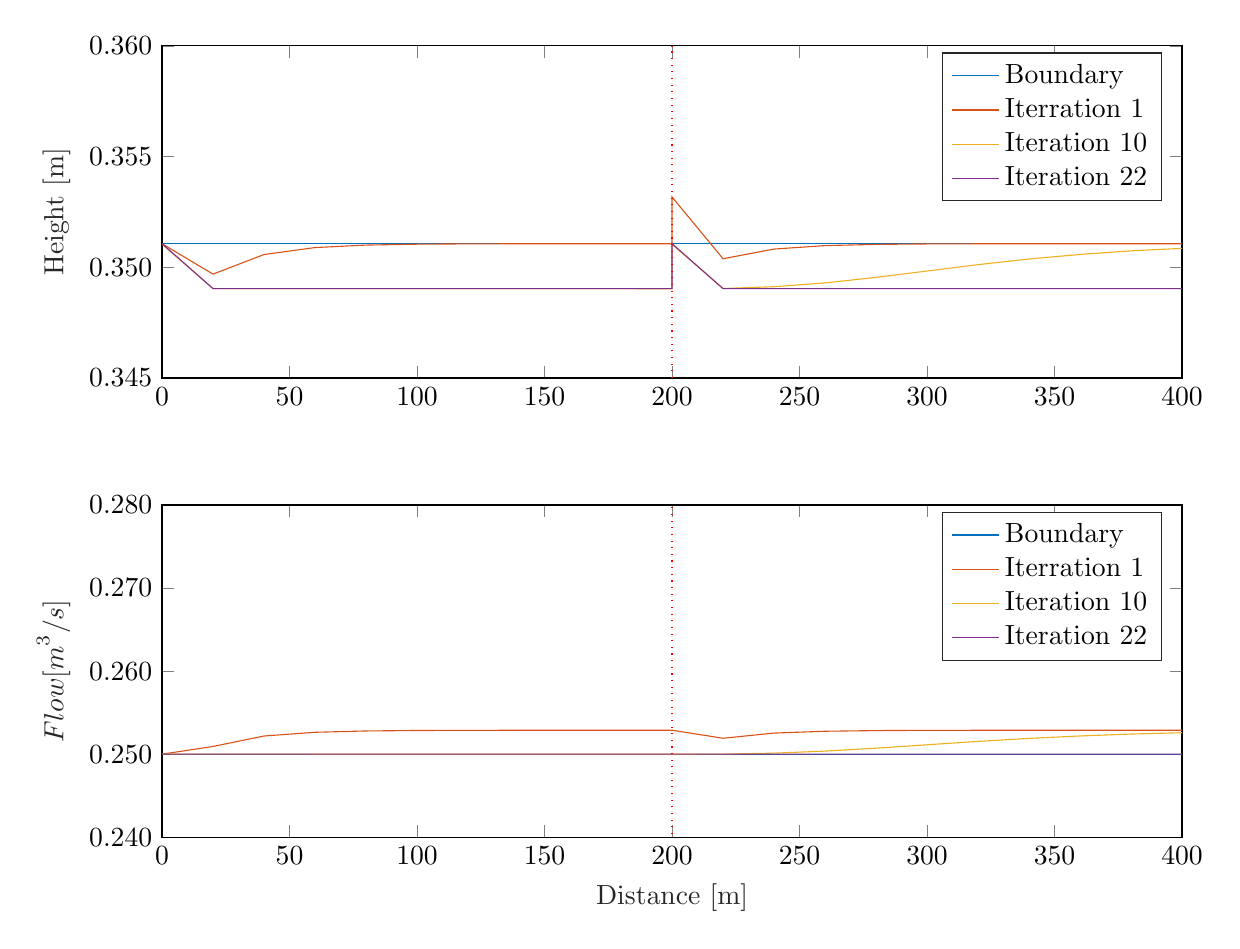
\begin{tikzpicture}

\begin{axis}[%
width=5.1in,
height=1.661in,
at={(2.08in,3.154in)},
scale only axis,
xmin=0,
xmax=400,
xlabel style={font=\color{white!15!black}},
%xlabel={Distance [m]},
ymin=0.345,
ymax=0.36,
ylabel style={font=\color{white!15!black}},
ylabel={Height [m]},
axis background/.style={fill=white},
y tick label style={
        /pgf/number format/.cd,
            fixed,
            fixed zerofill,
            precision=3,
        /tikz/.cd  },
title style={font=\bfseries},
%title={Curvefit},
legend style={legend cell align=left, align=left, draw=white!15!black}
]
\addplot [color=mycolor1]
  table[row sep=crcr]{%
0	0.351064698342896\\
200	0.351064698342896\\
400	0.351064698342896\\
};
\addlegendentry{Boundary}

\addplot [color=mycolor2]
  table[row sep=crcr]{%
0	0.351064698342896\\
20	0.349690425371762\\
40	0.350575480853252\\
60	0.350890269562512\\
80	0.351002475151802\\
100	0.351042501121412\\
120	0.351056775490292\\
140	0.351061870368596\\
200	0.351064571998904\\
200	0.35317394090697\\
220	0.350385544412916\\
240	0.350822634043709\\
260	0.350978353573737\\
280	0.351033892189093\\
300	0.351053708086965\\
320	0.351060775514213\\
360	0.351064199156951\\
400	0.351064634411387\\
};
\addlegendentry{Iterration 1}

\addplot [color=mycolor3]
  table[row sep=crcr]{%
0	0.351046566681021\\
20	0.349036521512801\\
180	0.349035279823624\\
200	0.349026739276496\\
200	0.35103637024929\\
220	0.349041213224552\\
240	0.349123089812394\\
260	0.349294685503196\\
280	0.349543083040601\\
320	0.350118505975786\\
340	0.350374059351282\\
360	0.350579188303925\\
380	0.350742011157763\\
400	0.350854227957257\\
};
\addlegendentry{Iteration 10}

\addplot [color=mycolor4]
  table[row sep=crcr]{%
0	0.351064698342952\\
20	0.349036521507401\\
200	0.349036522122788\\
200	0.351064698342952\\
220	0.349036521507401\\
400	0.349036532325727\\
};
\addlegendentry{Iteration 22}

\addplot [color=red, dotted, forget plot]
  table[row sep=crcr]{%
200	0.344999999999999\\
200	0.360000000000014\\
};
\end{axis}

\begin{axis}[%
width=5.1in,
height=1.661in,
at={(2.08in,0.858in)},
scale only axis,
xmin=0,
xmax=400,
xlabel style={font=\color{white!15!black}},
xlabel={Distance [m]},
ymin=0.24,
ymax=0.28,
ylabel style={font=\color{white!15!black}},
ylabel={$\text{Flow [m}^\text{3}\text{/s]}$},
y tick label style={
        /pgf/number format/.cd,
            fixed,
            fixed zerofill,
            precision=3,
        /tikz/.cd  },
axis background/.style={fill=white},
legend style={legend cell align=left, align=left, draw=white!15!black}
]
\addplot [color=mycolor1]
  table[row sep=crcr]{%
0	0.25\\
200	0.25\\
400	0.25\\
};
\addlegendentry{Boundary}

\addplot [color=mycolor2]
  table[row sep=crcr]{%
0	0.25\\
20	0.250927811672625\\
40	0.252185983866809\\
60	0.252634142815168\\
80	0.252793964154193\\
100	0.252850978285323\\
140	0.25287858109607\\
200	0.252882427974328\\
220	0.251915745479664\\
240	0.252537816935785\\
260	0.252759602617687\\
280	0.252838721204057\\
300	0.252866948997394\\
340	0.25288061725945\\
400	0.252882518538513\\
};
\addlegendentry{Iterration 1}

\addplot [color=mycolor3]
  table[row sep=crcr]{%
0	0.25\\
200	0.249986131352046\\
220	0.25000665171865\\
240	0.250122746526756\\
260	0.250366131411454\\
280	0.25071862987113\\
320	0.251536029676629\\
340	0.251899416890069\\
360	0.252191266279397\\
380	0.252423028186058\\
400	0.252582810584272\\
};
\addlegendentry{Iteration 10}

\addplot [color=mycolor4]
  table[row sep=crcr]{%
0	0.25\\
200	0.25\\
400	0.250000020948733\\
};
\addlegendentry{Iteration 22}

\addplot [color=red, dotted, forget plot]
  table[row sep=crcr]{%
200	0.22999999999999\\
200	0.300000000000011\\
};
\end{axis}
\end{tikzpicture}%
\caption{Height and flow in two adjoining pipes, with identical specifications given in table \ref{tab:pipe_figure_parameters}, given boundary conditions found by fitted polynomial, and calculated at various amount of iterations with constant flow input of 0,25 $\text{m}^\text{3}$/s. The dotted line indicates an intersection between pipes.}
\label{fig:two_pipes_init_steady_state}
\end{figure}

In figure \ref{fig:two_pipes_init_steady_state} a maximum of 22 iterations are performed. The iterations are stopped as the error between the input flow of 0,25 $\text{m}^\text{3}$/s desired to be in all sections, and the calculated flow in all the sections of the two pipes is less than $1\cdot10^{-7}$, which is a preset condition. 
Some discrepancy in heights can be seen at the start of both pipes. These two points are the boundary conditions that are found by the fitted polynomial. Even though the anomalies are small they could pose a problem when expanding the simulation with more pipes and different slopes. 

In figure \ref{fig:Fredericia_pipe_setup} the specifications of the main line of Fredericia mentioned in section \ref{se:system_description}, and given by table \ref{tab:kloak_diameter} with corrections from table \ref{tab:new_slope_values}, is seen.

\begin{figure}[H]
\centering
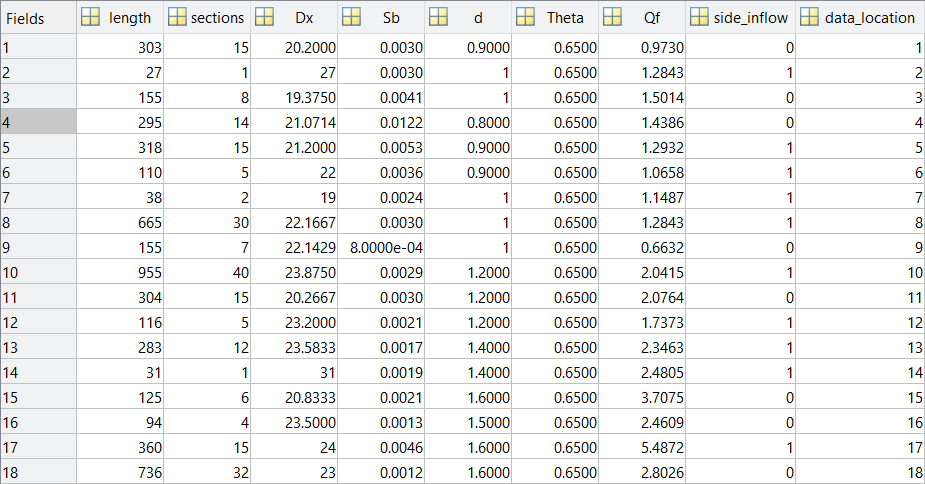
\includegraphics[width=0.97 \textwidth]{report/simulation/pictures/Fredericia_pipe_setup2.PNG}
\caption{Setup in MATLAB of pipe system from section \ref{se:system_description} of the main line in Fredericia.}
\label{fig:Fredericia_pipe_setup}
\end{figure}

The amount of sections for each pipe is chosen such that each section is close to being 20 meters, with some sections deviating due to pipe length and others deviate on purpose to see if it affects the outcome.  
To lessen the design complexity of the simulation environment a limitation is made on side input. It is decided that side input should not consist of pipes in which flow should be simulated. Instead it is chosen that side input is given from premade flow profiles. 
There is not given any side inflow in the results show in the following figures, as the indication of side inflow listed in figure \ref{fig:Fredericia_pipe_setup} just indicates the possibility of inflow to be given at the inlet of the pipe. 
In figure \ref{fig:fredericia_init_steady_state} iterations of the pipe setup shown in figure \ref{fig:Fredericia_pipe_setup} is seen. 




\begin{figure}[H]
 \centering
 % This file was created by matlab2tikz.
%
%The latest updates can be retrieved from
%  http://www.mathworks.com/matlabcentral/fileexchange/22022-matlab2tikz-matlab2tikz
%where you can also make suggestions and rate matlab2tikz.
%
\definecolor{mycolor1}{rgb}{0.00000,0.44700,0.74100}%
\definecolor{mycolor2}{rgb}{0.85000,0.32500,0.09800}%
\definecolor{mycolor3}{rgb}{0.92900,0.69400,0.12500}%
\definecolor{mycolor4}{rgb}{0.49400,0.18400,0.55600}%
%
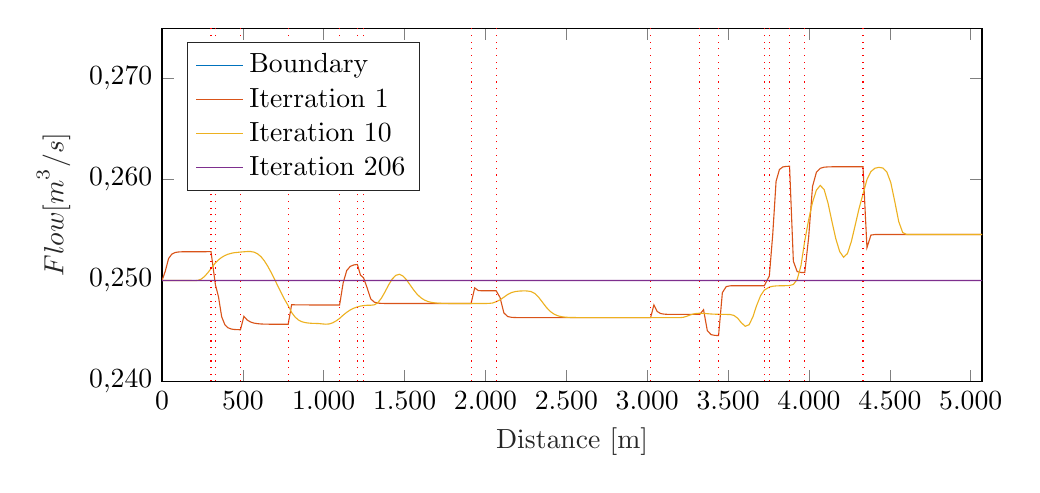
\begin{tikzpicture}

% \begin{axis}[%
% width=4.1in,
% height=1.7661in,
% at={(2.08in,4.154in)},
% scale only axis,
% xmin=0,
% xmax=5070,
% xlabel style={font=\color{white!15!black}},
% xlabel={Distance [m]},
% ymin=0.23,
% ymax=0.5,
% ylabel style={font=\color{white!15!black}},
% ylabel={Height [m]},
% y tick label style={
%         /pgf/number format/.cd,
%             fixed,
%             fixed zerofill,
%             precision=3,
%         /tikz/.cd  },
% axis background/.style={fill=white},
% title style={font=\bfseries},
% %title={Curvefit},
% legend style={legend cell align=left, align=left, draw=white!15!black}
% ]
% \addplot [color=mycolor1]
%   table[row sep=crcr]{%
% 0	0.351046566681362\\
% 303	0.351046566681362\\
% 303	0.335846494096586\\
% 330	0.335846494096586\\
% 330	0.309081835974212\\
% 485	0.309081835974212\\
% 485	0.252859425031602\\
% 780	0.252859425031602\\
% 780	0.30113200759115\\
% 1098	0.30113200759115\\
% 1098	0.334449091811621\\
% 1208	0.334449091811621\\
% 1208	0.356846112954372\\
% 1246	0.356846112954372\\
% 1246	0.335846494096586\\
% 1911	0.335846494096586\\
% 1911	0.471158308282611\\
% 2066	0.471158308282611\\
% 2066	0.31921912278267\\
% 3021	0.31921912278267\\
% 3021	0.316751000824297\\
% 3325	0.316751000824297\\
% 3325	0.344573805215077\\
% 3441	0.344573805215077\\
% 3441	0.349812515584745\\
% 3724	0.349812515584745\\
% 3724	0.341336368817792\\
% 3755	0.341336368817792\\
% 3755	0.326099272523606\\
% 3880	0.326099272523606\\
% 3880	0.366998098881595\\
% 3974	0.366998098881595\\
% 3974	0.268429914892295\\
% 4334	0.268429914892295\\
% 4334	0.369764380792731\\
% 5070	0.369764380792731\\
% };
% \addlegendentry{Boundary}

% \addplot [color=mycolor2]
%   table[row sep=crcr]{%
% 0	0.351046566681362\\
% 20.1999999999998	0.34968895516522\\
% 40.3999999999996	0.350569191323302\\
% 60.6000000000004	0.350878440171073\\
% 80.8000000000002	0.350987324814923\\
% 121.2	0.351039206755559\\
% 303	0.351046566320292\\
% 303	0.337920017091164\\
% 330	0.337104830155113\\
% 330	0.308816288287744\\
% 349.375	0.311112987536944\\
% 368.75	0.309891138768762\\
% 388.125	0.309403535853562\\
% 407.5	0.309209591216131\\
% 426.875	0.309132551677067\\
% 485	0.309085006824716\\
% 485	0.250256817505033\\
% 506.071428571428	0.253261105530328\\
% 527.142857142857	0.253071711576922\\
% 548.214285714286	0.25297158569083\\
% 590.357142857143	0.252890721389122\\
% 695.714285714286	0.25286070441507\\
% 780	0.252859526163775\\
% 780	0.29830065184251\\
% 801.2	0.301150556440007\\
% 907.2	0.30113221456395\\
% 1098	0.301132007618435\\
% 1098	0.332701121968967\\
% 1120	0.333213670339319\\
% 1142	0.334029438639845\\
% 1164	0.334306307291627\\
% 1186	0.334400486116465\\
% 1208	0.334432545507298\\
% 1208	0.358081245261019\\
% 1227	0.357124156438658\\
% 1246	0.356938719651225\\
% 1246	0.336046212403744\\
% 1268.16666666667	0.3368923261296\\
% 1290.33333333333	0.336155393261834\\
% 1312.5	0.335937573806405\\
% 1334.66666666667	0.335873335453471\\
% 1401.16666666667	0.335847180709607\\
% 1911	0.335846494096586\\
% 1911	0.469052641075905\\
% 1933.14285714286	0.471444240967685\\
% 1955.28571428571	0.471182537374261\\
% 2021.71428571429	0.471158322977317\\
% 2066	0.471158308388112\\
% 2066	0.318622019097347\\
% 2089.875	0.320496612934221\\
% 2113.75	0.319514616894594\\
% 2137.625	0.319287270193854\\
% 2185.375	0.319222740165969\\
% 2591.25	0.31921912278267\\
% 3021	0.31921912278267\\
% 3021	0.314621592146977\\
% 3041.26666666667	0.31734996286832\\
% 3061.53333333333	0.316937914631126\\
% 3081.8	0.31680927511843\\
% 3122.33333333333	0.316756658182385\\
% 3325	0.316751001048033\\
% 3325	0.342308375285029\\
% 3348.2	0.346359256224787\\
% 3371.4	0.344919252401269\\
% 3394.6	0.344640318741767\\
% 3441	0.344576265712021\\
% 3441	0.346419453900126\\
% 3464.58333333333	0.34933410965732\\
% 3488.16666666667	0.349748600842759\\
% 3511.75	0.349803954984964\\
% 3676.83333333333	0.349812515087251\\
% 3724	0.349812515511985\\
% 3724	0.341028456009553\\
% 3755	0.340964073333453\\
% 3755	0.326379126597203\\
% 3775.83333333333	0.321868331375299\\
% 3796.66666666667	0.325179423238296\\
% 3817.5	0.325897210955191\\
% 3838.33333333333	0.326054795641539\\
% 3880	0.326097118924736\\
% 3880	0.374240674311295\\
% 3903.5	0.36780783584345\\
% 3927	0.367066436455389\\
% 3950.5	0.367003841449332\\
% 3974	0.366998570777469\\
% 3974	0.268879357493461\\
% 3998	0.264827740485089\\
% 4022	0.267433813811294\\
% 4046	0.268152302385715\\
% 4070	0.268352371899709\\
% 4118	0.268423854368848\\
% 4334	0.26842991391004\\
% 4334	0.376983027044844\\
% 4358.53333333333	0.36882153381157\\
% 4383.06666666667	0.369723472334044\\
% 4432.13333333333	0.369764301605755\\
% 5070	0.369764380792731\\
% };
% \addlegendentry{Iterration 1}

% \addplot [color=mycolor3]
%   table[row sep=crcr]{%
% 0	0.351046566681362\\
% 20.1999999999998	0.349036521511152\\
% 222.2	0.349046405044646\\
% 242.4	0.34913649455757\\
% 262.6	0.34931781803607\\
% 303	0.349867060769611\\
% 303	0.336702948036873\\
% 330	0.33855939613295\\
% 330	0.310203922742403\\
% 349.375	0.313399640052921\\
% 388.125	0.31365882096361\\
% 426.875	0.313795071539062\\
% 485	0.313873335364406\\
% 485	0.254360830428595\\
% 506.071428571428	0.256514049001453\\
% 548.214285714286	0.256525580034577\\
% 569.285714285715	0.256494061431113\\
% 590.357142857143	0.256412516409\\
% 611.428571428572	0.25627214218639\\
% 632.5	0.256062121847208\\
% 674.642857142857	0.25547654307411\\
% 780	0.253803281379987\\
% 780	0.29950777787144\\
% 801.2	0.300683487595052\\
% 822.400000000001	0.300405720608069\\
% 843.6	0.300226905975251\\
% 864.8	0.300123006869399\\
% 907.2	0.300040684715896\\
% 1013.2	0.299972975182754\\
% 1034.4	0.299989670735158\\
% 1055.6	0.300057473315974\\
% 1098	0.300324088652815\\
% 1098	0.331736350766732\\
% 1120	0.331058913244306\\
% 1164	0.33140846830247\\
% 1208	0.331607801616883\\
% 1208	0.354810386877944\\
% 1227	0.354927732049873\\
% 1246	0.354962121926292\\
% 1246	0.334037440969951\\
% 1268.16666666667	0.335729443493619\\
% 1312.5	0.335756541749106\\
% 1334.66666666667	0.335902203338264\\
% 1356.83333333333	0.336208190886282\\
% 1423.33333333333	0.337484250179841\\
% 1445.5	0.337729710069652\\
% 1467.66666666667	0.337798281448158\\
% 1489.83333333333	0.337684513221575\\
% 1512	0.337423827597377\\
% 1578.5	0.336452942219694\\
% 1600.66666666667	0.336230470627015\\
% 1622.83333333333	0.336076415241223\\
% 1667.16666666667	0.335918079838848\\
% 1733.66666666667	0.335855917980552\\
% 1911	0.33584650892135\\
% 1911	0.469052661346723\\
% 1933.14285714286	0.4699077760406\\
% 2021.71428571429	0.469917536872344\\
% 2043.85714285714	0.469957208950291\\
% 2066	0.470084055845291\\
% 2066	0.317987071485732\\
% 2089.875	0.320345312932659\\
% 2137.625	0.320690256576199\\
% 2161.5	0.320810702687595\\
% 2209.25	0.320904038049775\\
% 2257	0.320910505313805\\
% 2280.875	0.320874020298106\\
% 2304.75	0.320754183039753\\
% 2328.625	0.320512047461307\\
% 2376.375	0.319869753429884\\
% 2400.25	0.31961347737797\\
% 2424.125	0.319438155648641\\
% 2448	0.319332029334873\\
% 2495.75	0.319244099456228\\
% 2591.25	0.319219847591739\\
% 3021	0.319219122783579\\
% 3021	0.314621592146977\\
% 3041.26666666667	0.316548539435644\\
% 3223.66666666667	0.316569082669957\\
% 3304.73333333333	0.316813070417993\\
% 3325	0.316823754671532\\
% 3325	0.342385574041145\\
% 3348.2	0.346106817103646\\
% 3441	0.346045061387485\\
% 3441	0.347733336406236\\
% 3464.58333333333	0.347834659294676\\
% 3511.75	0.347824145261256\\
% 3535.33333333333	0.347763516550003\\
% 3558.91666666667	0.347569185570137\\
% 3582.5	0.347245649706565\\
% 3606.08333333333	0.347008957041908\\
% 3629.66666666667	0.347112454168382\\
% 3653.25	0.347662697129635\\
% 3676.83333333333	0.348455924252448\\
% 3700.41666666667	0.349115411154344\\
% 3724	0.349509151722486\\
% 3724	0.340766113725294\\
% 3755	0.340213352281353\\
% 3755	0.325705016530264\\
% 3775.83333333333	0.318653120913041\\
% 3838.33333333333	0.318687704680087\\
% 3880	0.318699569309501\\
% 3880	0.366677469372007\\
% 3903.5	0.366143421387278\\
% 3927	0.366498551967197\\
% 3950.5	0.367493250538246\\
% 3974	0.369271682220642\\
% 3974	0.270655412324231\\
% 3998	0.265735491228952\\
% 4022	0.266631554775813\\
% 4046	0.267245120456209\\
% 4070	0.267486938321781\\
% 4094	0.267270537983677\\
% 4118	0.26657699736279\\
% 4142	0.265646627718525\\
% 4166	0.264762694837373\\
% 4190	0.264105549345004\\
% 4214	0.263816377362673\\
% 4238	0.264005547972374\\
% 4262	0.264621496441578\\
% 4310	0.266321059502843\\
% 4334	0.2670422870724\\
% 4334	0.375262946422481\\
% 4358.53333333333	0.373659708724517\\
% 4383.06666666667	0.374227586426969\\
% 4407.6	0.374456751804246\\
% 4432.13333333333	0.374521854303566\\
% 4456.66666666667	0.37447392642116\\
% 4481.2	0.37420123087486\\
% 4505.73333333333	0.373451103634579\\
% 4530.26666666667	0.372122015676723\\
% 4554.8	0.370693736438625\\
% 4579.33333333333	0.369906031144637\\
% 4603.86666666667	0.369767004346613\\
% 4800.13333333333	0.36976437955127\\
% 5070	0.369764380792731\\
% };
% \addlegendentry{Iteration 10}

% \addplot [color=mycolor4]
%   table[row sep=crcr]{%
% 0	0.351046566681362\\
% 20.1999999999998	0.349036521511152\\
% 303	0.349036522123242\\
% 303	0.335846494096586\\
% 330	0.337383528097234\\
% 330	0.309081835974212\\
% 349.375	0.312127255888299\\
% 485	0.312127255888299\\
% 485	0.252859425031602\\
% 506.071428571428	0.255070955894553\\
% 780	0.25507095868943\\
% 780	0.30113200759115\\
% 801.2	0.302597885206524\\
% 1098	0.302597889182834\\
% 1098	0.334449091811621\\
% 1120	0.333365463585324\\
% 1208	0.333365460573987\\
% 1208	0.356846112954372\\
% 1227	0.356742349043088\\
% 1246	0.356742349043088\\
% 1246	0.335846494096586\\
% 1268.16666666667	0.337383528097234\\
% 1911	0.337383528097234\\
% 1911	0.471158308282611\\
% 1933.14285714286	0.472168027992666\\
% 2066	0.472168027992666\\
% 2066	0.31921912278267\\
% 2089.875	0.321570501145288\\
% 3021	0.321570503379917\\
% 3021	0.316751000824297\\
% 3041.26666666667	0.318880063902725\\
% 3325	0.318880065802659\\
% 3325	0.344573805215077\\
% 3348.2	0.348367030399459\\
% 3441	0.348367034072908\\
% 3441	0.349812515584745\\
% 3464.58333333333	0.350168554430638\\
% 3724	0.350168562385988\\
% 3724	0.341336368817792\\
% 3755	0.340652282182418\\
% 3755	0.326099272523606\\
% 3775.83333333333	0.319013731798805\\
% 3880	0.319013719205032\\
% 3880	0.366998098881595\\
% 3903.5	0.366424696740069\\
% 3974	0.366424680770251\\
% 3974	0.268429914892295\\
% 3998	0.26261486783369\\
% 4334	0.262614857666449\\
% 4334	0.369764380792731\\
% 4358.53333333333	0.366466763596691\\
% 5070	0.366466931269315\\
% };
% \addlegendentry{Iteration 206}

% \addplot [color=red, dotted, forget plot]
%   table[row sep=crcr]{%
% 303	0.230000000000018\\
% 303	0.5\\
% };
% \addplot [color=red, dotted, forget plot]
%   table[row sep=crcr]{%
% 330	0.230000000000018\\
% 330	0.5\\
% };
% \addplot [color=red, dotted, forget plot]
%   table[row sep=crcr]{%
% 485	0.230000000000018\\
% 485	0.5\\
% };
% \addplot [color=red, dotted, forget plot]
%   table[row sep=crcr]{%
% 780	0.230000000000018\\
% 780	0.5\\
% };
% \addplot [color=red, dotted, forget plot]
%   table[row sep=crcr]{%
% 1098	0.230000000000018\\
% 1098	0.5\\
% };
% \addplot [color=red, dotted, forget plot]
%   table[row sep=crcr]{%
% 1208	0.230000000000018\\
% 1208	0.5\\
% };
% \addplot [color=red, dotted, forget plot]
%   table[row sep=crcr]{%
% 1246	0.230000000000018\\
% 1246	0.5\\
% };
% \addplot [color=red, dotted, forget plot]
%   table[row sep=crcr]{%
% 1911	0.230000000000018\\
% 1911	0.5\\
% };
% \addplot [color=red, dotted, forget plot]
%   table[row sep=crcr]{%
% 2066	0.230000000000018\\
% 2066	0.5\\
% };
% \addplot [color=red, dotted, forget plot]
%   table[row sep=crcr]{%
% 3021	0.230000000000018\\
% 3021	0.5\\
% };
% \addplot [color=red, dotted, forget plot]
%   table[row sep=crcr]{%
% 3325	0.230000000000018\\
% 3325	0.5\\
% };
% \addplot [color=red, dotted, forget plot]
%   table[row sep=crcr]{%
% 3441	0.230000000000018\\
% 3441	0.5\\
% };
% \addplot [color=red, dotted, forget plot]
%   table[row sep=crcr]{%
% 3724	0.230000000000018\\
% 3724	0.5\\
% };
% \addplot [color=red, dotted, forget plot]
%   table[row sep=crcr]{%
% 3755	0.230000000000018\\
% 3755	0.5\\
% };
% \addplot [color=red, dotted, forget plot]
%   table[row sep=crcr]{%
% 3880	0.230000000000018\\
% 3880	0.5\\
% };
% \addplot [color=red, dotted, forget plot]
%   table[row sep=crcr]{%
% 3974	0.230000000000018\\
% 3974	0.5\\
% };
% \addplot [color=red, dotted, forget plot]
%   table[row sep=crcr]{%
% 4334	0.229999999999563\\
% 4334	0.5\\
% };
% \end{axis}

\begin{axis}[%
/pgf/number format/1000 sep={.},/pgf/number format/use comma,
width=4.1in,
height=1.7661in,
at={(2.08in,0.858in)},
scale only axis,
xmin=0,
xmax=5070,
xlabel style={font=\color{white!15!black}},
xlabel={Distance [m]},
ymin=0.24,
ymax=0.275,
ylabel style={font=\color{white!15!black}},
ylabel={$\text{Flow [m}^\text{3}\text{/s]}$},
y tick label style={
        /pgf/number format/.cd,
            fixed,
            fixed zerofill,
            precision=3,
        /tikz/.cd  },
axis background/.style={fill=white},
legend style={legend cell align=left, align=left, draw=white!15!black},
legend style={at={(0.03,0.75)},anchor=west}
]
\addplot [color=mycolor1]
  table[row sep=crcr]{%
0	0.25\\
303	0.25\\
330	0.25\\
485	0.25\\
780	0.25\\
1098	0.25\\
1208	0.25\\
1246	0.25\\
1911	0.25\\
2066	0.25\\
3021	0.25\\
3325	0.25\\
3441	0.25\\
3724	0.25\\
3755	0.25\\
3880	0.25\\
3974	0.25\\
4334	0.25\\
5070	0.25\\
};
\addlegendentry{Boundary}

\addplot [color=mycolor2]
  table[row sep=crcr]{%
0	0.25\\
20.1999999999998	0.250925723985347\\
40.3999999999996	0.252177033286898\\
60.6000000000004	0.252617295405798\\
80.8000000000002	0.252772381408249\\
101	0.252827029878972\\
121.2	0.252846289461559\\
161.6	0.2528554748842\\
303	0.252856777308807\\
330	0.249586439912491\\
349.375	0.248369130628816\\
368.75	0.246411360997627\\
388.125	0.245632173439844\\
407.5	0.245322583773486\\
426.875	0.245199659832906\\
446.25	0.245150865513097\\
465.625	0.245131498819319\\
485	0.245123812414931\\
506.071428571428	0.246448496023731\\
527.142857142857	0.246078273970852\\
548.214285714286	0.245882648810948\\
569.285714285715	0.245779299061724\\
590.357142857143	0.245724705487191\\
611.428571428572	0.245695874536977\\
632.5	0.245680649383758\\
674.642857142857	0.24566835045789\\
758.928571428572	0.245663970916212\\
780	0.245663792863525\\
801.2	0.24760942885132\\
822.400000000001	0.247591338313214\\
864.8	0.247580934929829\\
970.8	0.247578878983404\\
1098	0.247578855406573\\
1120	0.249773608390569\\
1142	0.250991365916889\\
1164	0.251405278094353\\
1186	0.251546136946672\\
1208	0.251594088487764\\
1227	0.25053424781072\\
1246	0.250274708132565\\
1268.16666666667	0.249271322087225\\
1290.33333333333	0.2481799954503\\
1312.5	0.247857858795214\\
1334.66666666667	0.24776289341753\\
1356.83333333333	0.247734908463826\\
1379	0.247726662622881\\
1445.5	0.247723306276384\\
1911	0.247723218172723\\
1933.14285714286	0.249270184074703\\
1955.28571428571	0.249006471097346\\
1977.42857142857	0.248984126917094\\
2043.85714285714	0.248982061816605\\
2066	0.248982060669732\\
2089.875	0.248318521606052\\
2113.75	0.246785884586643\\
2137.625	0.246431718725034\\
2161.5	0.246350060716395\\
2185.375	0.246331245551119\\
2233.125	0.24632591651789\\
2758.375	0.246325606637583\\
3021	0.246325606637583\\
3041.26666666667	0.247585553451245\\
3061.53333333333	0.2469373616741\\
3081.8	0.246735165330392\\
3102.06666666667	0.246672136071538\\
3122.33333333333	0.246652495763556\\
3162.86666666667	0.246644465559257\\
3325	0.246643597168259\\
3348.2	0.247105149917843\\
3371.4	0.24503914725392\\
3394.6	0.244639948356962\\
3417.8	0.244563105193265\\
3441	0.244548324589232\\
3464.58333333333	0.248798997152335\\
3488.16666666667	0.249395180864667\\
3511.75	0.24947486857036\\
3535.33333333333	0.249485538243789\\
3629.66666666667	0.249487194905669\\
3724	0.249487203114768\\
3755	0.250462095202238\\
3775.83333333333	0.254532530491815\\
3796.66666666667	0.25984168605919\\
3817.5	0.260999984299815\\
3838.33333333333	0.261254608546551\\
3859.16666666667	0.261310673363369\\
3880	0.261323023638397\\
3903.5	0.251908495744829\\
3927	0.25088460558618\\
3950.5	0.250798250835032\\
3974	0.250791006868894\\
3998	0.25425993321096\\
4022	0.259323709164164\\
4046	0.260728674673373\\
4070	0.261120604514872\\
4094	0.261230108759264\\
4118	0.261260720106293\\
4142	0.261269272221398\\
4214	0.261272523807747\\
4334	0.261272615673988\\
4358.53333333333	0.253252944457017\\
4383.06666666667	0.254504559788984\\
4407.6	0.254558913653455\\
4481.2	0.254561432057926\\
5070	0.254561444401588\\
};
\addlegendentry{Iterration 1}

\addplot [color=mycolor3]
  table[row sep=crcr]{%
0	0.25\\
181.8	0.249997570520463\\
202	0.249986793087373\\
222.2	0.250014005769117\\
242.4	0.250141755574077\\
262.6	0.250398949418923\\
282.8	0.250763051554713\\
303	0.25117870521899\\
330	0.251748425060214\\
349.375	0.252053211283055\\
368.75	0.25229191895869\\
388.125	0.252472440840393\\
407.5	0.252602860122352\\
426.875	0.252692963639674\\
446.25	0.252756247452453\\
485	0.252819676466061\\
527.142857142857	0.252874228651308\\
548.214285714286	0.252872146506888\\
569.285714285715	0.252809755454109\\
590.357142857143	0.252648349750416\\
611.428571428572	0.252370614871325\\
632.5	0.25195533711485\\
653.571428571428	0.251419542777512\\
674.642857142857	0.25079923548401\\
695.714285714286	0.250127155533846\\
716.785714285715	0.249431478053339\\
737.857142857143	0.24874203377658\\
758.928571428572	0.24809140717116\\
780	0.247509845702552\\
801.2	0.246840276889088\\
822.400000000001	0.246383403959044\\
843.6	0.246089493381078\\
864.8	0.245918800557774\\
886	0.24582814297446\\
907.2	0.245783596140427\\
928.400000000001	0.245755316632312\\
949.6	0.245748068348803\\
970.8	0.245734425434421\\
992	0.245699663582855\\
1013.2	0.245672418333925\\
1034.4	0.245699829891237\\
1055.6	0.24581117048092\\
1076.8	0.246003437515355\\
1098	0.246249214930685\\
1120	0.246569866557365\\
1142	0.246854916452321\\
1164	0.247088334512227\\
1186	0.247262881142888\\
1208	0.247384204231821\\
1227	0.247468046954054\\
1246	0.247515921229933\\
1268.16666666667	0.247550236255847\\
1290.33333333333	0.247550128305193\\
1312.5	0.247590278027928\\
1334.66666666667	0.247805567502837\\
1356.83333333333	0.248258108455047\\
1379	0.248887572368403\\
1401.16666666667	0.249571083247247\\
1423.33333333333	0.2501495410188\\
1445.5	0.250514149332048\\
1467.66666666667	0.250616050609096\\
1489.83333333333	0.250446994723461\\
1512	0.250059827184486\\
1556.33333333333	0.249053454950626\\
1578.5	0.24862036468312\\
1600.66666666667	0.248291074359258\\
1622.83333333333	0.248063170760361\\
1645	0.247917017099098\\
1667.16666666667	0.247829038492455\\
1689.33333333333	0.247778837759142\\
1711.5	0.247751477483689\\
1733.66666666667	0.247737147636144\\
1778	0.247726345462979\\
1866.66666666667	0.247723340563425\\
1911	0.247723240085179\\
1999.57142857143	0.247724554827073\\
2021.71428571429	0.247733041258471\\
2043.85714285714	0.247772945277575\\
2066	0.247900547897189\\
2089.875	0.248082064429582\\
2113.75	0.248348098605675\\
2137.625	0.248621282349632\\
2161.5	0.248809712509683\\
2185.375	0.248910617275214\\
2209.25	0.248955783601559\\
2233.125	0.24897184153815\\
2257	0.248965905636396\\
2280.875	0.248908809586283\\
2304.75	0.248721300688885\\
2328.625	0.248342653318105\\
2376.375	0.24733960192134\\
2400.25	0.246939953201036\\
2424.125	0.246666746413212\\
2448	0.246501428645388\\
2471.875	0.246410610971907\\
2495.75	0.246364509708656\\
2519.625	0.246342587930485\\
2543.5	0.246332719202655\\
2591.25	0.246326738868447\\
2782.25	0.246325608631196\\
3021	0.246325606638493\\
3203.4	0.246320864111112\\
3223.66666666667	0.246357856887698\\
3243.93333333333	0.246455281891031\\
3264.2	0.246578717228658\\
3284.46666666667	0.246681971252656\\
3304.73333333333	0.246741121185551\\
3325	0.246757907916617\\
3348.2	0.246742343738333\\
3394.6	0.24668361638669\\
3417.8	0.246664545527892\\
3441	0.246653628356398\\
3511.75	0.246633161628779\\
3535.33333333333	0.246546398517239\\
3558.91666666667	0.246268394425897\\
3582.5	0.24580595626594\\
3606.08333333333	0.245467899489086\\
3629.66666666667	0.245615703122894\\
3653.25	0.246402196250529\\
3676.83333333333	0.247538197913855\\
3700.41666666667	0.248484714096776\\
3724	0.249050687163617\\
3755	0.249350220121414\\
3775.83333333333	0.249430362921885\\
3796.66666666667	0.249465302152203\\
3817.5	0.249479221503861\\
3859.16666666667	0.249489592804821\\
3880	0.249503750157601\\
3903.5	0.249612794999848\\
3927	0.250101761113001\\
3950.5	0.251473788065596\\
3974	0.253936247960155\\
3998	0.256018005487931\\
4022	0.257759468026961\\
4046	0.258955347088886\\
4070	0.2594274388548\\
4094	0.259005016269839\\
4118	0.257653327917978\\
4142	0.255845672541\\
4166	0.254134246225476\\
4190	0.252865715890039\\
4214	0.252308499922947\\
4238	0.25267289277599\\
4262	0.253861350384796\\
4286	0.255495515304574\\
4310	0.257155356047406\\
4334	0.258559689078538\\
4358.53333333333	0.260003321073782\\
4383.06666666667	0.260801603624714\\
4407.6	0.261124074209874\\
4432.13333333333	0.261215637287023\\
4456.66666666667	0.26114818096994\\
4481.2	0.260764462199404\\
4505.73333333333	0.259710435672787\\
4530.26666666667	0.257848166359508\\
4554.8	0.255854459096554\\
4579.33333333333	0.254758339201544\\
4603.86666666667	0.254565136389829\\
4628.4	0.25455690722265\\
4677.46666666667	0.254561219286188\\
5070	0.254561444401588\\
};
\addlegendentry{Iteration 10}

\addplot [color=mycolor4]
  table[row sep=crcr]{%
0	0.25\\
303	0.25\\
330	0.25\\
485	0.25\\
780	0.25\\
1098	0.25\\
1208	0.25\\
1246	0.25\\
1911	0.25\\
2066	0.25\\
3021	0.25\\
3325	0.25\\
3441	0.25\\
3724	0.25\\
3755	0.25\\
3880	0.25\\
3974	0.25\\
4334	0.25\\
5070	0.25000028087652\\
};
\addlegendentry{Iteration 206}

\addplot [color=red, dotted, forget plot]
  table[row sep=crcr]{%
303	0.240000000000009\\
303	0.274999999999982\\
};
\addplot [color=red, dotted, forget plot]
  table[row sep=crcr]{%
330	0.240000000000009\\
330	0.274999999999982\\
};
\addplot [color=red, dotted, forget plot]
  table[row sep=crcr]{%
485	0.240000000000009\\
485	0.274999999999982\\
};
\addplot [color=red, dotted, forget plot]
  table[row sep=crcr]{%
780	0.240000000000009\\
780	0.274999999999982\\
};
\addplot [color=red, dotted, forget plot]
  table[row sep=crcr]{%
1098	0.240000000000009\\
1098	0.274999999999982\\
};
\addplot [color=red, dotted, forget plot]
  table[row sep=crcr]{%
1208	0.240000000000009\\
1208	0.274999999999982\\
};
\addplot [color=red, dotted, forget plot]
  table[row sep=crcr]{%
1246	0.240000000000009\\
1246	0.274999999999982\\
};
\addplot [color=red, dotted, forget plot]
  table[row sep=crcr]{%
1911	0.240000000000009\\
1911	0.274999999999982\\
};
\addplot [color=red, dotted, forget plot]
  table[row sep=crcr]{%
2066	0.239999999999782\\
2066	0.274999999999982\\
};
\addplot [color=red, dotted, forget plot]
  table[row sep=crcr]{%
3021	0.239999999999782\\
3021	0.274999999999982\\
};
\addplot [color=red, dotted, forget plot]
  table[row sep=crcr]{%
3325	0.239999999999782\\
3325	0.274999999999982\\
};
\addplot [color=red, dotted, forget plot]
  table[row sep=crcr]{%
3441	0.239999999999782\\
3441	0.274999999999982\\
};
\addplot [color=red, dotted, forget plot]
  table[row sep=crcr]{%
3724	0.239999999999782\\
3724	0.274999999999982\\
};
\addplot [color=red, dotted, forget plot]
  table[row sep=crcr]{%
3755	0.239999999999782\\
3755	0.274999999999982\\
};
\addplot [color=red, dotted, forget plot]
  table[row sep=crcr]{%
3880	0.239999999999782\\
3880	0.274999999999982\\
};
\addplot [color=red, dotted, forget plot]
  table[row sep=crcr]{%
3974	0.239999999999782\\
3974	0.274999999999982\\
};
\addplot [color=red, dotted, forget plot]
  table[row sep=crcr]{%
4334	0.239999999999782\\
4334	0.274999999999982\\
};
\end{axis}
\end{tikzpicture}%
\caption{Height and flow of pipe setup from part of Fredericia, given by table \ref{tab:kloak_diameter} with corrections from table \ref{tab:new_slope_values}, where boundary conditions is found by fitted polynomial. Various amount of iterations, with constant flow input of 0,25 $\text{m}^\text{3}$/s, is performed. The dotted line indicates pipe intersections.}
\label{fig:fredericia_init_steady_state}
\end{figure}

It is clear that the larger setup increases the undesired behavior seen in figure \ref{fig:two_pipes_init_steady_state}. But it can also be seen that the flow can be brought to an acceptable initial state from which the system can start simulating. In figure \ref{fig:fredericia_init_steady_state_zoom} a section of the height plot from figure \ref{fig:fredericia_init_steady_state} is seen. 
% system needs to be brought in to steady state to negate unintended results when starting simulating.

\begin{figure}[H]
 \centering
 % This file was created by matlab2tikz.
%
%The latest updates can be retrieved from
%  http://www.mathworks.com/matlabcentral/fileexchange/22022-matlab2tikz-matlab2tikz
%where you can also make suggestions and rate matlab2tikz.
%
\definecolor{mycolor1}{rgb}{0.00000,0.44700,0.74100}%
\definecolor{mycolor2}{rgb}{0.85000,0.32500,0.09800}%
%
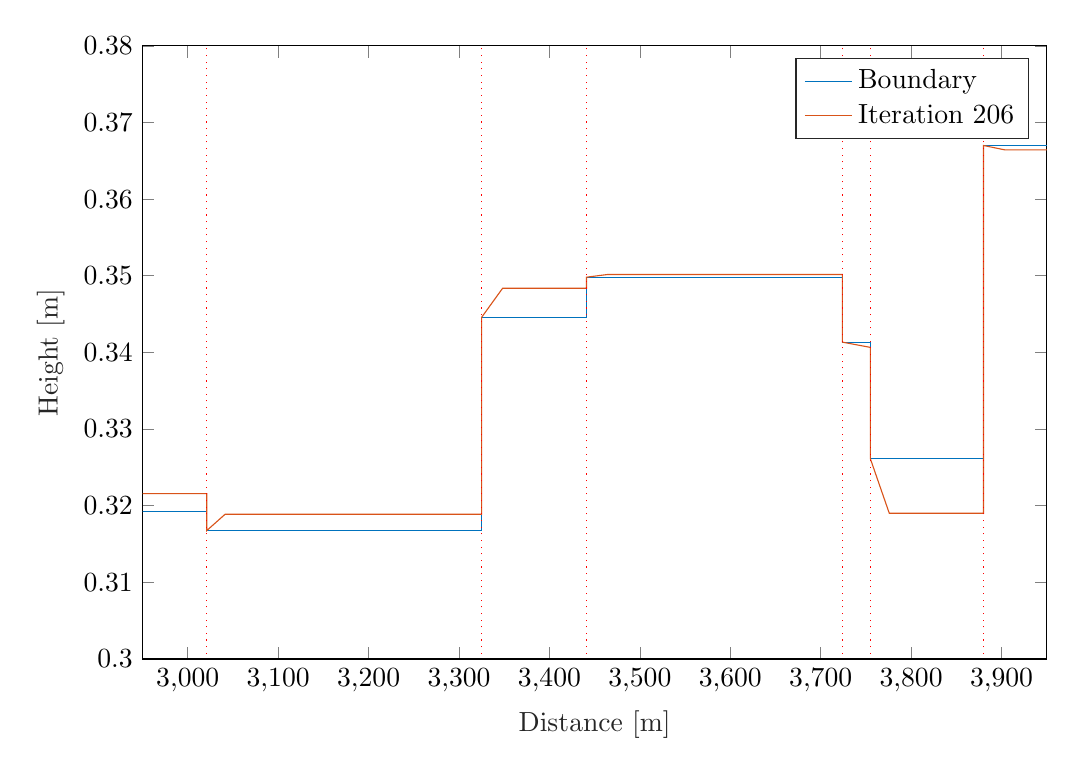
\begin{tikzpicture}

\begin{axis}[%
width=4.521in,
height=3.066in,
at={(0.758in,0.481in)},
scale only axis,
xmin=2950,
xmax=3950,
xlabel style={font=\color{white!15!black}},
xlabel={Distance [m]},
ymin=0.3,
ymax=0.38,
ylabel style={font=\color{white!15!black}},
ylabel={Height [m]},
axis background/.style={fill=white},
title style={font=\bfseries},
%title={Curvefit},
legend style={legend cell align=left, align=left, draw=white!15!black}
]
\addplot [color=mycolor1]
  table[row sep=crcr]{%
2949.375	0.31921912278267\\
3021	0.31921912278267\\
3021	0.316751000824752\\
3325	0.316751000824752\\
3325	0.344573805214623\\
3441	0.344573805214623\\
3441	0.34981251558429\\
3724	0.34981251558429\\
3724	0.341336368817338\\
3755	0.341336368817338\\
3755	0.326099272523606\\
3880	0.326099272523606\\
3880	0.366998098881595\\
3950.5	0.366998098881595\\
};
\addlegendentry{Boundary}

\addplot [color=mycolor2]
  table[row sep=crcr]{%
2949.375	0.321570503379462\\
3021	0.321570503379462\\
3021	0.316751000824752\\
3041.26666666667	0.318880063902725\\
3325	0.318880065802659\\
3325	0.344573805214623\\
3348.2	0.348367030399004\\
3441	0.348367034072908\\
3441	0.34981251558429\\
3464.58333333333	0.350168554431093\\
3724	0.350168562385988\\
3724	0.341336368817338\\
3755	0.340652282182418\\
3755	0.326099272523606\\
3775.83333333333	0.319013731799259\\
3880	0.319013719205032\\
3880	0.366998098881595\\
3903.5	0.366424696740069\\
3950.5	0.366424682920751\\
};
\addlegendentry{Iteration 206}

\addplot [color=red, dotted, forget plot]
  table[row sep=crcr]{%
3021	0.291999999999916\\
3021	0.38799999999992\\
};
\addplot [color=red, dotted, forget plot]
  table[row sep=crcr]{%
3325	0.291999999999916\\
3325	0.38799999999992\\
};
\addplot [color=red, dotted, forget plot]
  table[row sep=crcr]{%
3441	0.291999999999916\\
3441	0.38799999999992\\
};
\addplot [color=red, dotted, forget plot]
  table[row sep=crcr]{%
3724	0.291999999999916\\
3724	0.38799999999992\\
};
\addplot [color=red, dotted, forget plot]
  table[row sep=crcr]{%
3755	0.291999999999916\\
3755	0.38799999999992\\
};
\addplot [color=red, dotted, forget plot]
  table[row sep=crcr]{%
3880	0.291999999999916\\
3880	0.38799999999992\\
};
\end{axis}
\end{tikzpicture}%
\caption{Segment of the height plot shown in figure \ref{fig:fredericia_init_steady_state}. Pipe 10 and 16 is seen partially at the left and right side and 11 to 15 in between with a red stippled line separating pipes.}
\label{fig:fredericia_init_steady_state_zoom}
\end{figure}
In the above figure, the obtained height from the fitted polynomial is at it worst off by almost a centimeter. But when simulating this offset will only occur in the first section of the pipe. This means that it will be a greater disturbance on short pipes with few sections than larger ones with more sections. An alternative method is attempted to conclude if the deviations of the curve fitted polynomial seen in figure \ref{fig:curvefit_comparision_split} is the cause or if there is an unforeseen error in the Preissmann scheme. A lookup table, where the same data used to create the polynomial, is utilized. A simple implementation is made where the index in the vector of flow is found by subtracting the input flow from the vector. The desired index is then found by searching for the lowest absolute value. Finally the resulting height is given as the desired index of the height vector. The chosen scheme for creating the lookup table means that the height will in the worst case be rounded to the nearest step. But indexing the flow and height into the chosen 10.000 steps, it is assumed to be an insignificant error, and in the worst case the number of steps can be increased. In figure \ref{fig:fredericia_init_steady_state_lut} an identical test of the pipe setup of Fredericia is performed at various iterations.      

\begin{figure}[H]
 \centering
 % This file was created by matlab2tikz.
%
%The latest updates can be retrieved from
%  http://www.mathworks.com/matlabcentral/fileexchange/22022-matlab2tikz-matlab2tikz
%where you can also make suggestions and rate matlab2tikz.
%
\definecolor{mycolor1}{rgb}{0.00000,0.44700,0.74100}%
\definecolor{mycolor2}{rgb}{0.85000,0.32500,0.09800}%
\definecolor{mycolor3}{rgb}{0.92900,0.69400,0.12500}%
\definecolor{mycolor4}{rgb}{0.49400,0.18400,0.55600}%
%
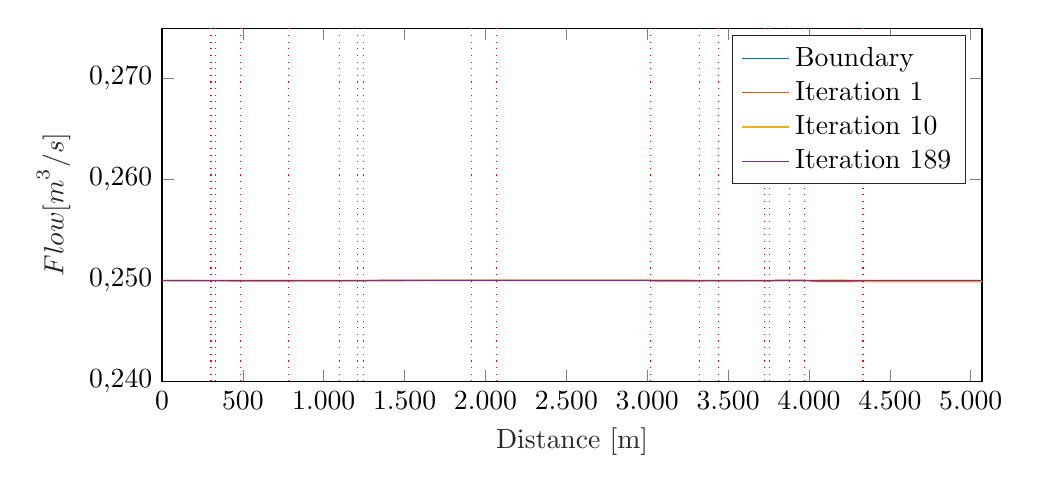
\begin{tikzpicture}

% \begin{axis}[%
% width=5.1in,
% height=2.661in,
% at={(2.08in,4.154in)},
% scale only axis,
% xmin=0,
% xmax=5070,
% xlabel style={font=\color{white!15!black}},
% xlabel={Distance [m]},
% ymin=0.23,
% ymax=0.5,
% ylabel style={font=\color{white!15!black}},
% ylabel={Height [m]},
% y tick label style={
%         /pgf/number format/.cd,
%             fixed,
%             fixed zerofill,
%             precision=3,
%         /tikz/.cd  },
% axis background/.style={fill=white},
% title style={font=\bfseries},
% title={Lookup table},
% legend style={legend cell align=left, align=left, draw=white!15!black}
% ]
% \addplot [color=mycolor1]
%   table[row sep=crcr]{%
% 0	0.349019999999655\\
% 303	0.349019999999655\\
% 303	0.337400000000343\\
% 330	0.337400000000343\\
% 330	0.3121000000001\\
% 485	0.3121000000001\\
% 485	0.255040000000008\\
% 780	0.255040000000008\\
% 780	0.30257999999958\\
% 1098	0.30257999999958\\
% 1098	0.33335999999963\\
% 1208	0.33335999999963\\
% 1208	0.356700000000274\\
% 1246	0.356700000000274\\
% 1246	0.337400000000343\\
% 1911	0.337400000000343\\
% 1911	0.472200000000157\\
% 2066	0.472200000000157\\
% 2066	0.321600000000217\\
% 3021	0.321600000000217\\
% 3021	0.318839999999909\\
% 3325	0.318839999999909\\
% 3325	0.348359999999957\\
% 3441	0.348359999999957\\
% 3441	0.350139999999556\\
% 3724	0.350139999999556\\
% 3724	0.340619999999944\\
% 3755	0.340619999999944\\
% 3755	0.319040000000314\\
% 3880	0.319040000000314\\
% 3880	0.366450000000441\\
% 3974	0.366450000000441\\
% 3974	0.262560000000121\\
% 4334	0.262560000000121\\
% 4334	0.366399999999885\\
% 5070	0.366399999999885\\
% };
% \addlegendentry{Boundary}

% \addplot [color=mycolor2]
%   table[row sep=crcr]{%
% 0	0.349019999999655\\
% 80.8000000000002	0.349020481316074\\
% 303	0.349020000000564\\
% 303	0.337400000000343\\
% 330	0.337380589420718\\
% 330	0.3121000000001\\
% 368.75	0.312106867829243\\
% 485	0.312100028022542\\
% 485	0.255040000000008\\
% 611.428571428572	0.255040284774623\\
% 780	0.255040001183261\\
% 780	0.30257999999958\\
% 843.6	0.302577760769054\\
% 1098	0.302579999983209\\
% 1098	0.33335999999963\\
% 1186	0.333359622993157\\
% 1208	0.333359874085545\\
% 1208	0.356700000000274\\
% 1246	0.356708069378328\\
% 1246	0.337400000000343\\
% 1268.16666666667	0.337368396814782\\
% 1334.66666666667	0.337399179543354\\
% 1911	0.337400000000343\\
% 1911	0.472200000000157\\
% 2066	0.472199999998338\\
% 2066	0.321600000000217\\
% 2257	0.321599999286263\\
% 3021	0.321600000000217\\
% 3021	0.318959999999606\\
% 3041.26666666667	0.318844345599246\\
% 3325	0.318840000006276\\
% 3325	0.348359999999957\\
% 3371.4	0.348355689153323\\
% 3441	0.348359969182638\\
% 3441	0.350139999999556\\
% 3511.75	0.350140224120878\\
% 3724	0.350140000011379\\
% 3724	0.340619999999944\\
% 3755	0.340622273461122\\
% 3755	0.319040000000314\\
% 3775.83333333333	0.319007018123557\\
% 3817.5	0.319038499465933\\
% 3880	0.319039982874529\\
% 3880	0.366450000000441\\
% 3974	0.366450006908963\\
% 3974	0.262560000000121\\
% 3998	0.262606505555596\\
% 4046	0.262563473184855\\
% 4334	0.262560000153826\\
% 4334	0.366399999999885\\
% 4530.26666666667	0.366399999871646\\
% 5070	0.366399999999885\\
% };
% \addlegendentry{Iterration 1}

% \addplot [color=mycolor3]
%   table[row sep=crcr]{%
% 0	0.349019999999655\\
% 60.6000000000004	0.349036522010465\\
% 303	0.349029645651171\\
% 303	0.337400000000343\\
% 330	0.337375436085495\\
% 330	0.3121000000001\\
% 388.125	0.312116053602949\\
% 485	0.312113124059579\\
% 485	0.255040000000008\\
% 548.214285714286	0.255059158875156\\
% 780	0.255055547565462\\
% 780	0.30257999999958\\
% 1098	0.302564515821359\\
% 1098	0.33335999999963\\
% 1142	0.333332646147028\\
% 1208	0.333340608369326\\
% 1208	0.356700000000274\\
% 1246	0.356718336754966\\
% 1246	0.337400000000343\\
% 1290.33333333333	0.337362335213584\\
% 1911	0.337399999565605\\
% 1911	0.472200000000157\\
% 2043.85714285714	0.472192406379691\\
% 2066	0.472192812377216\\
% 2066	0.321600000000217\\
% 2161.5	0.321588994348531\\
% 3021	0.321600000000217\\
% 3021	0.318959999999606\\
% 3041.26666666667	0.318909314883058\\
% 3304.73333333333	0.318869159727001\\
% 3325	0.318859556761709\\
% 3325	0.348359999999957\\
% 3394.6	0.348327480761327\\
% 3441	0.348324021764711\\
% 3441	0.350139999999556\\
% 3511.75	0.350125604256391\\
% 3724	0.350143100147761\\
% 3724	0.340619999999944\\
% 3755	0.340626457929829\\
% 3755	0.319040000000314\\
% 3775.83333333333	0.318989076884463\\
% 3880	0.318987695751275\\
% 3880	0.366450000000441\\
% 3903.5	0.366394930784736\\
% 3974	0.366409957899123\\
% 3974	0.262560000000121\\
% 4022	0.262614928369658\\
% 4214	0.262630593074391\\
% 4334	0.262577626555867\\
% 4334	0.366399999999885\\
% 4432.13333333333	0.36639104866299\\
% 5070	0.366399999999885\\
% };
% \addlegendentry{Iteration 10}

% \addplot [color=mycolor4]
%   table[row sep=crcr]{%
% 0	0.349019999999655\\
% 60.6000000000004	0.349036522010465\\
% 303	0.349036522123242\\
% 303	0.337400000000343\\
% 330	0.337383528097234\\
% 330	0.3121000000001\\
% 368.75	0.312127255888299\\
% 485	0.312127255888299\\
% 485	0.255040000000008\\
% 527.142857142857	0.255070957815406\\
% 780	0.25507095868943\\
% 780	0.30257999999958\\
% 843.6	0.302597889077333\\
% 1098	0.302597889182834\\
% 1098	0.33335999999963\\
% 1208	0.333365460569439\\
% 1208	0.356700000000274\\
% 1246	0.356742349043088\\
% 1246	0.337400000000343\\
% 1312.5	0.337383528097234\\
% 1911	0.337383528097234\\
% 1911	0.472200000000157\\
% 1955.28571428571	0.472168027992666\\
% 2066	0.472168027992666\\
% 2066	0.321600000000217\\
% 2113.75	0.321570504886949\\
% 3021	0.321570503379917\\
% 3021	0.318839999999909\\
% 3061.53333333333	0.318880063972756\\
% 3325	0.318880065802659\\
% 3325	0.348359999999957\\
% 3441	0.348367034051989\\
% 3441	0.350139999999556\\
% 3488.16666666667	0.350168559149097\\
% 3724	0.350168562385988\\
% 3724	0.340619999999944\\
% 3755	0.340652255206805\\
% 3755	0.319040000000314\\
% 3796.66666666667	0.319013727231322\\
% 3880	0.319013719325085\\
% 3880	0.366450000000441\\
% 3927	0.366424689039377\\
% 3974	0.366424681146782\\
% 3974	0.262560000000121\\
% 3998	0.262614845033568\\
% 4334	0.26261485766554\\
% 4334	0.366399999999885\\
% 4358.53333333333	0.366466726264662\\
% 5070	0.366466605791175\\
% };
% \addlegendentry{Iteration 189}

% \addplot [color=red, dotted, forget plot]
%   table[row sep=crcr]{%
% 303	0.230000000000018\\
% 303	0.5\\
% };
% \addplot [color=red, dotted, forget plot]
%   table[row sep=crcr]{%
% 330	0.230000000000018\\
% 330	0.5\\
% };
% \addplot [color=red, dotted, forget plot]
%   table[row sep=crcr]{%
% 485	0.230000000000018\\
% 485	0.5\\
% };
% \addplot [color=red, dotted, forget plot]
%   table[row sep=crcr]{%
% 780	0.230000000000018\\
% 780	0.5\\
% };
% \addplot [color=red, dotted, forget plot]
%   table[row sep=crcr]{%
% 1098	0.230000000000018\\
% 1098	0.5\\
% };
% \addplot [color=red, dotted, forget plot]
%   table[row sep=crcr]{%
% 1208	0.230000000000018\\
% 1208	0.5\\
% };
% \addplot [color=red, dotted, forget plot]
%   table[row sep=crcr]{%
% 1246	0.230000000000018\\
% 1246	0.5\\
% };
% \addplot [color=red, dotted, forget plot]
%   table[row sep=crcr]{%
% 1911	0.230000000000018\\
% 1911	0.5\\
% };
% \addplot [color=red, dotted, forget plot]
%   table[row sep=crcr]{%
% 2066	0.230000000000018\\
% 2066	0.5\\
% };
% \addplot [color=red, dotted, forget plot]
%   table[row sep=crcr]{%
% 3021	0.230000000000018\\
% 3021	0.5\\
% };
% \addplot [color=red, dotted, forget plot]
%   table[row sep=crcr]{%
% 3325	0.230000000000018\\
% 3325	0.5\\
% };
% \addplot [color=red, dotted, forget plot]
%   table[row sep=crcr]{%
% 3441	0.230000000000018\\
% 3441	0.5\\
% };
% \addplot [color=red, dotted, forget plot]
%   table[row sep=crcr]{%
% 3724	0.230000000000018\\
% 3724	0.5\\
% };
% \addplot [color=red, dotted, forget plot]
%   table[row sep=crcr]{%
% 3755	0.230000000000018\\
% 3755	0.5\\
% };
% \addplot [color=red, dotted, forget plot]
%   table[row sep=crcr]{%
% 3880	0.230000000000018\\
% 3880	0.5\\
% };
% \addplot [color=red, dotted, forget plot]
%   table[row sep=crcr]{%
% 3974	0.230000000000018\\
% 3974	0.5\\
% };
% \addplot [color=red, dotted, forget plot]
%   table[row sep=crcr]{%
% 4334	0.229999999999563\\
% 4334	0.5\\
% };
% \end{axis}

\begin{axis}[%
/pgf/number format/1000 sep={.},/pgf/number format/use comma,
width=4.1in,
height=1.7661in,
at={(2.08in,0.858in)},
scale only axis,
xmin=0,
xmax=5070,
xlabel style={font=\color{white!15!black}},
xlabel={Distance [m]},
ymin=0.24,
ymax=0.275,
ylabel style={font=\color{white!15!black}},
ylabel={$\text{Flow [m}^\text{3}\text{/s]}$},
y tick label style={
        /pgf/number format/.cd,
            fixed,
            fixed zerofill,
            precision=3,
        /tikz/.cd  },
axis background/.style={fill=white},
legend style={legend cell align=left, align=left, draw=white!15!black}
]
\addplot [color=mycolor1]
  table[row sep=crcr]{%
0	0.25\\
303	0.25\\
330	0.25\\
485	0.25\\
780	0.25\\
1098	0.25\\
1208	0.25\\
1246	0.25\\
1911	0.25\\
2066	0.25\\
3021	0.25\\
3325	0.25\\
3441	0.25\\
3724	0.25\\
3755	0.25\\
3880	0.25\\
3974	0.25\\
4334	0.25\\
5070	0.25\\
};
\addlegendentry{Boundary}

\addplot [color=mycolor2]
  table[row sep=crcr]{%
0	0.25\\
60.6000000000004	0.249978522559104\\
181.8	0.249976578495989\\
303	0.249976576241352\\
330	0.249995637611391\\
388.125	0.249960527929943\\
446.25	0.249956389295221\\
485	0.249956152021696\\
590.357142857143	0.249940082209832\\
780	0.249939045288556\\
843.6	0.24996667841333\\
928.400000000001	0.249970279605805\\
1098	0.249970385933921\\
1164	0.249990196854014\\
1208	0.249991662936736\\
1246	0.249952059458337\\
1268.16666666667	0.249977538387611\\
1290.33333333333	0.25001056144356\\
1312.5	0.25002033943565\\
1379	0.250024345979909\\
1911	0.250024452777325\\
1977.42857142857	0.250032223487324\\
2066	0.250032254260077\\
2137.625	0.250045787679483\\
2543.5	0.25004626554346\\
3021	0.25004626554346\\
3041.26666666667	0.249943509264085\\
3081.8	0.24993731453651\\
3325	0.249936628178148\\
3371.4	0.24998358783705\\
3417.8	0.249989579559042\\
3441	0.249989769594322\\
3488.16666666667	0.249961217600685\\
3582.5	0.249958852517011\\
3724	0.249958843491186\\
3755	0.249955586868964\\
3775.83333333333	0.249989375663972\\
3796.66666666667	0.250030383417652\\
3817.5	0.250039139651562\\
3880	0.250041486897317\\
3974	0.250034890455026\\
3998	0.249984011331435\\
4022	0.249919238147413\\
4046	0.24990154439547\\
4094	0.249895386285061\\
4334	0.249894859729466\\
4407.6	0.249908068946752\\
5070	0.249908105777649\\
};
\addlegendentry{Iteration 1}

\addplot [color=mycolor3]
  table[row sep=crcr]{%
0	0.25\\
262.6	0.249996705091689\\
303	0.249990246794368\\
330	0.249987987705936\\
485	0.249977241522174\\
780	0.249969651238644\\
864.8	0.249959840581141\\
1034.4	0.249941208218843\\
1098	0.249944758969832\\
1164	0.249955518235765\\
1208	0.249962931765367\\
1246	0.249966418070471\\
1401.16666666667	0.249976220261487\\
1467.66666666667	0.249981009654221\\
1512	0.249984605378813\\
1667.16666666667	0.250021862440917\\
1822.33333333333	0.250024434770239\\
1911	0.250024452131584\\
2066	0.250025003068004\\
2304.75	0.250033845017242\\
2495.75	0.250046057881264\\
3021	0.25004626554346\\
3223.66666666667	0.250044100288505\\
3243.93333333333	0.250034984778722\\
3325	0.24996756830933\\
3441	0.249937825736197\\
3535.33333333333	0.249941782698443\\
3582.5	0.249961131167765\\
3629.66666666667	0.249978221881975\\
3676.83333333333	0.249973853478878\\
3724	0.249963325268254\\
3755	0.249961808230182\\
3880	0.249958886077366\\
3927	0.249960381648634\\
3950.5	0.249966168777974\\
3974	0.249979746679855\\
3998	0.249986417225045\\
4070	0.250023586625503\\
4118	0.250034725949263\\
4190	0.250035535980714\\
4214	0.250030181091461\\
4238	0.250016839358977\\
4286	0.249970979716636\\
4334	0.249928669712972\\
4407.6	0.24989800178264\\
4481.2	0.249895426942203\\
4800.13333333333	0.249908105894974\\
5070	0.249908105777649\\
};
\addlegendentry{Iteration 10}

\addplot [color=mycolor4]
  table[row sep=crcr]{%
0	0.25\\
303	0.25\\
330	0.25\\
485	0.25\\
780	0.25\\
1098	0.25\\
1208	0.25\\
1246	0.25\\
1911	0.25\\
2066	0.25\\
3021	0.25\\
3325	0.25\\
3441	0.25\\
3724	0.25\\
3755	0.25\\
3880	0.25\\
3974	0.25\\
4334	0.25\\
5070	0.249999787922206\\
};
\addlegendentry{Iteration 189}

\addplot [color=red, dotted, forget plot]
  table[row sep=crcr]{%
303	0.240000000000009\\
303	0.274999999999977\\
};
\addplot [color=red, dotted, forget plot]
  table[row sep=crcr]{%
330	0.240000000000009\\
330	0.274999999999977\\
};
\addplot [color=red, dotted, forget plot]
  table[row sep=crcr]{%
485	0.240000000000009\\
485	0.274999999999977\\
};
\addplot [color=red, dotted, forget plot]
  table[row sep=crcr]{%
780	0.240000000000009\\
780	0.274999999999977\\
};
\addplot [color=red, dotted, forget plot]
  table[row sep=crcr]{%
1098	0.240000000000009\\
1098	0.275000000000091\\
};
\addplot [color=red, dotted, forget plot]
  table[row sep=crcr]{%
1208	0.240000000000009\\
1208	0.275000000000091\\
};
\addplot [color=red, dotted, forget plot]
  table[row sep=crcr]{%
1246	0.240000000000009\\
1246	0.275000000000091\\
};
\addplot [color=red, dotted, forget plot]
  table[row sep=crcr]{%
1911	0.240000000000009\\
1911	0.275000000000091\\
};
\addplot [color=red, dotted, forget plot]
  table[row sep=crcr]{%
2066	0.239999999999782\\
2066	0.275000000000091\\
};
\addplot [color=red, dotted, forget plot]
  table[row sep=crcr]{%
3021	0.239999999999782\\
3021	0.275000000000091\\
};
\addplot [color=red, dotted, forget plot]
  table[row sep=crcr]{%
3325	0.239999999999782\\
3325	0.275000000000091\\
};
\addplot [color=red, dotted, forget plot]
  table[row sep=crcr]{%
3441	0.239999999999782\\
3441	0.275000000000091\\
};
\addplot [color=red, dotted, forget plot]
  table[row sep=crcr]{%
3724	0.239999999999782\\
3724	0.275000000000091\\
};
\addplot [color=red, dotted, forget plot]
  table[row sep=crcr]{%
3755	0.239999999999782\\
3755	0.275000000000091\\
};
\addplot [color=red, dotted, forget plot]
  table[row sep=crcr]{%
3880	0.239999999999782\\
3880	0.275000000000091\\
};
\addplot [color=red, dotted, forget plot]
  table[row sep=crcr]{%
3974	0.239999999999782\\
3974	0.275000000000091\\
};
\addplot [color=red, dotted, forget plot]
  table[row sep=crcr]{%
4334	0.239999999999782\\
4334	0.274999999999636\\
};
\end{axis}
\end{tikzpicture}%
\caption{Height and flow of pipe setup from part of Fredericia, given by table \ref{tab:kloak_diameter} with corrections from table \ref{tab:new_slope_values}, where boundary conditions is found by lookup table. Various amount of iterations, with constant flow input of 0,25 $\text{m}^\text{3}$/s, is performed. The dotted line indicates pipe intersections.}
\label{fig:fredericia_init_steady_state_lut}
\end{figure}

It is clearly shown that the deviation between the boundary conditions found by the lookup table and the values found by the following iterations of the Preissmann scheme is significantly decreased.
Something else to note is that even though the difference seem to be non-existent it still required 189 iterations before the flow error was minimized to the same 1$\cdot \text{10}^{\text{-7}}$ as before. For this reason, it is decided to implement the scheme which brings the adjoining pipe parts into steady state before the simulation starts. A decisive choice is not made at this point whether the curve fitted polynomial or the lookup table should be implemented. The reason for this is that some imprecision can be accepted if reduction in simulation time can be obtained. A test will therefore be performed, in the simulation part of the implementation, to decided which scheme should be utilized. A flow chart of the initialization scheme, where initial values for the entire setup is found, can be seen in figure \ref{fig:init_sys_dia}.

\begin{figure}[H]
\centering
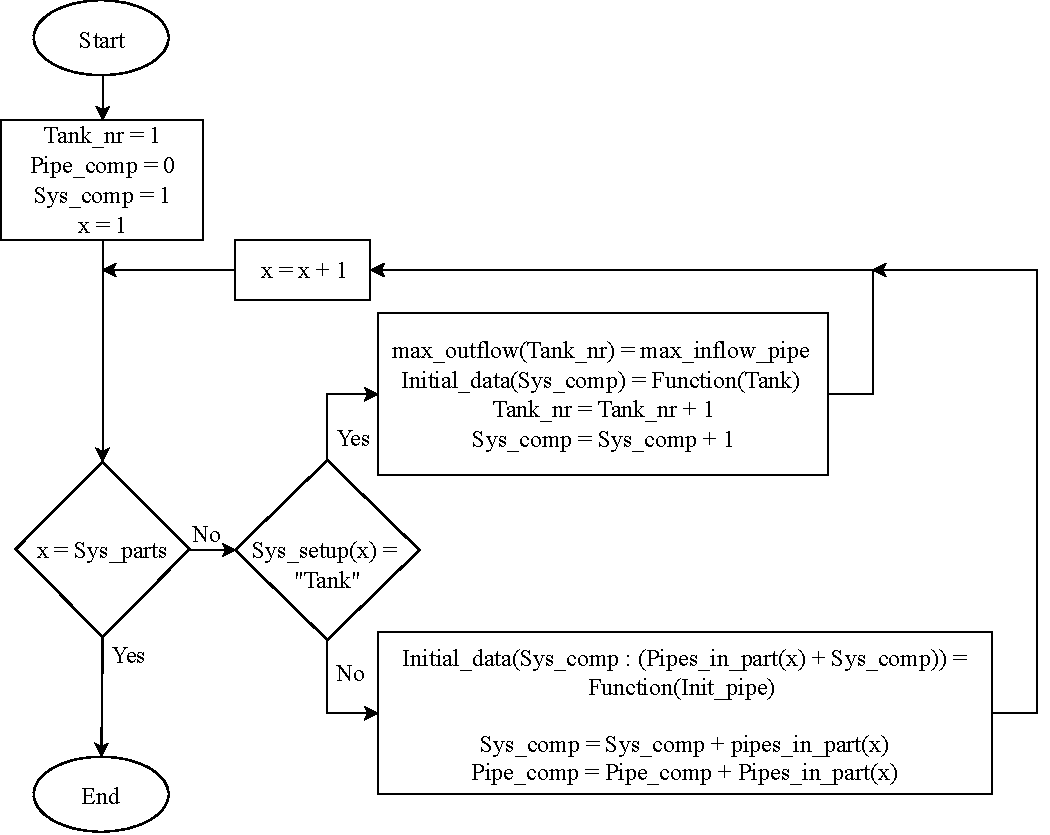
\includegraphics[width=1.05 \textwidth]{report/simulation/pictures/init_sys_dia.pdf}
\caption{Initialization loop.}
\label{fig:init_sys_dia}
\end{figure}

Two functions, namely ``Tank'' and ``Init\_pipe'', is used to obtain the initial values for tanks and the boundary conditions, for the pipes, needed to start iterating with the Preissmann scheme. The tank function returns the initial flow, height and the input needed for the pump, such that inflow is equal to outflow in the tank. Due to MPC requiring constraints for the input to the pump in the tank and due to time constraint of the project, a limitation in the simulation is made. The limitation refers to tanks not being able to be the end point of the entire system setup. The reason for this is that a uniform control input of zero to one for all pumps, to ease constraint setup when utilizing MPC, is obtained. The following parameters are set in the tank function:
\begin{itemize}
	\item $Q_{in} = Q_{initial}$ $[m^3/s]$
	\item $Q_{out} = Q_{in}$ $[m^3/s]$
	\item $u_{initial} = Q_{in}/Q_{max-outflow}$ $[\cdot]$
	\item $h = h_{initial}$ $[m]$
	\item $C = C_{initial}$ $[g/m^3]$
\end{itemize}

Where Q is flow, u is pump input, h is height and C is concentrate.
The pipe function is given initial flow, a component number from the system setup list in figure \ref{fig:sys_setup_matlab}, the corresponding pipe specifications to the number of pipes indicated by the system setup list and an error value. The error value is the accepted error between desired flow and the flow obtained by iterating with the Preissmann scheme, which means that when the error is less than the error value the system is in the desired steady state. A flowchart of the pipe function can be seen in figure \ref{fig:init_pipe_chart}. 

\begin{figure}[H]
\centering
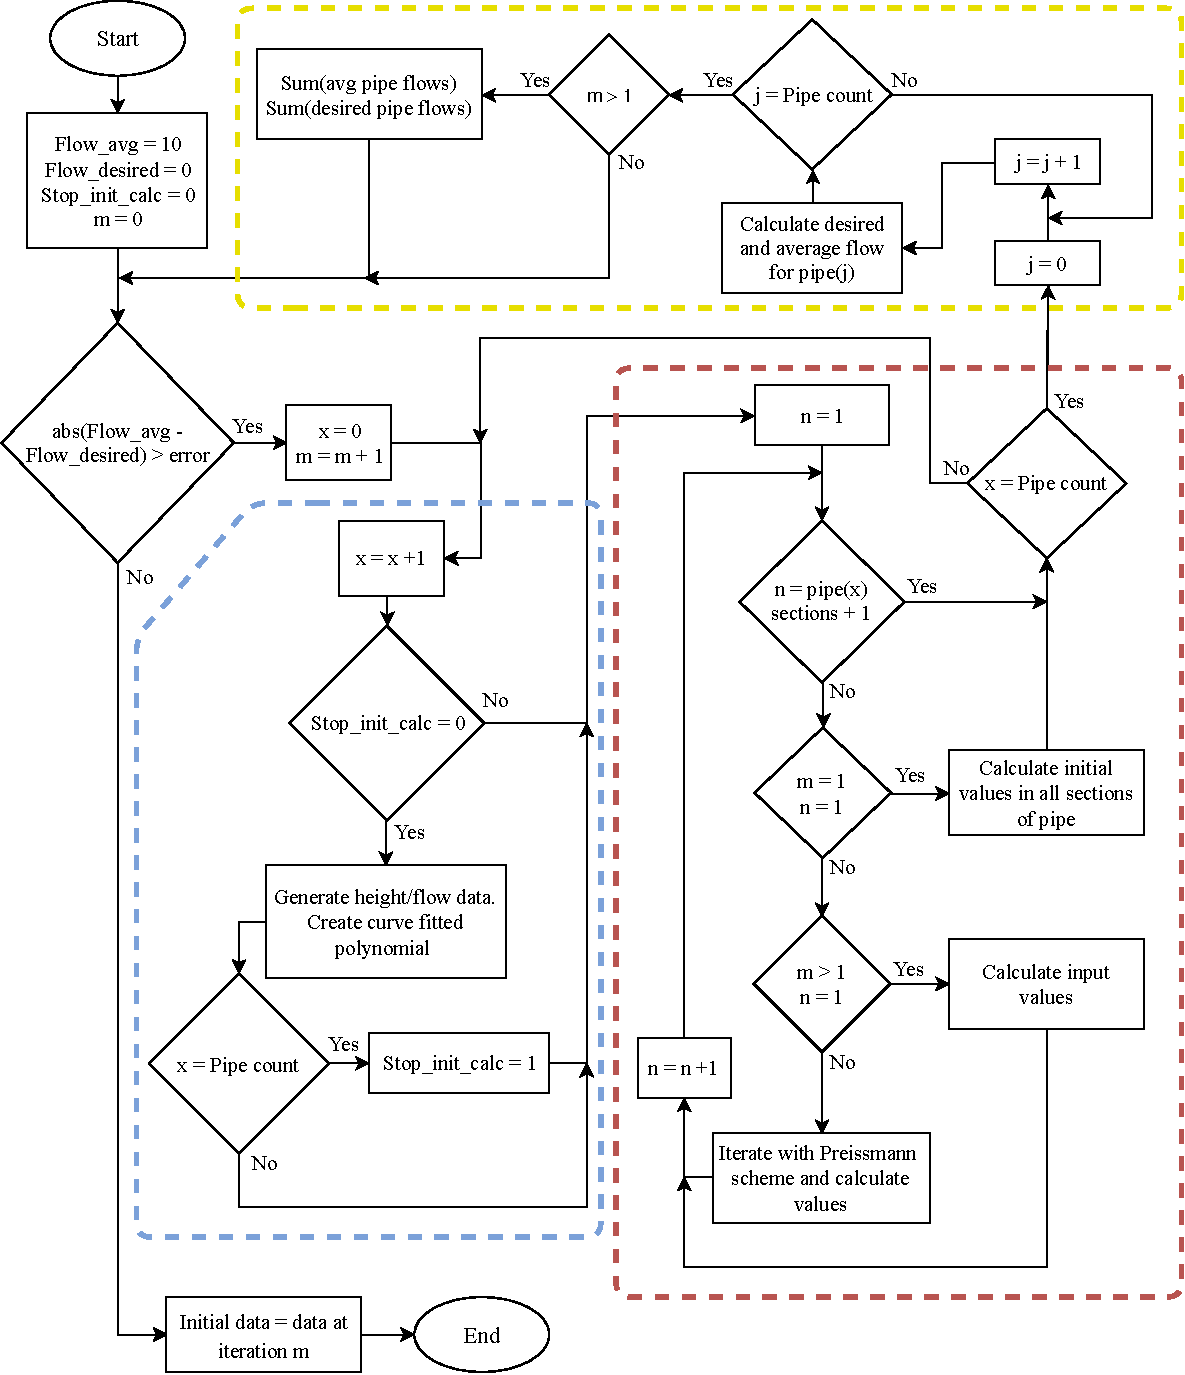
\includegraphics[width=1.05 \textwidth]{report/simulation/pictures/init_pipe_chart.pdf}
\caption{Flowchart of pipe initializing function where the blue box is the setup of the curve fitted polynomial for each pipe, the red box is the computation of data in pipes and the yellow box calculates desired and average flow for error stop condition. Furthermore ``x'' indicates a specific pipe, ``m'' is time step and ``n'' indicates the section in a pipe.}
\label{fig:init_pipe_chart}
\end{figure}

The pipe initialization function can be separated into three parts as indicated by the blue, red and yellow stippled boxes. In the blue stippled box the generated data, which can also be used for a lookup table, is used to create the curve fitted polynomial. When data are generated for all the pipes given to the function, a flag is set such that unnecessary calculations are not performed further on. 

In the red stippled box the calculations of the height and concentrate are performed. In the first time iteration ``m = 1'' the initial boundary condition is set for all sections of pipe number ``x''. This corresponds to the i-th row of circles shown in figure \ref{fig:preissmann_grid_scheme_exampel}. Furthermore, when iterating through the pipes the corresponding pipe specifications is checked to decide if the pipe has side inflow. If it is present then the inflow into the pipe is a simple summation of input flow and side inflow. The concentrate input in the case of side inflow is found by equation \ref{poop_addition_interconnection}. For the next pipe, the input is then set to be the output of the previous pipe plus eventual side inflow. At the following time iterations, the input boundary condition is found at section ``n = 1''. The Preissmann scheme is then utilized to find the height, and the concentrate is calculated, for the remaining pipe sections. This is done for all the pipes given to the function.

Lastly, in the yellow stippled box the desired and average flow values in the pipe or pipes are calculated. At the first time iteration ``m = 1'' the values of ``Flow\_avg'' and ``Flow\_desired'' are not updated. The reason is that the initial flow is inserted as the flow in all sections of all the pipes, which would give an error which is zero and stop the initialization loop. In the following iterations, disregarding the boundary condition which is still calculated, the flow is found from a height which can vary for some iterations as seen in figure \ref{fig:fredericia_init_steady_state}. When the flow in all sections of all the pipes has an error which is sufficiently small from the desired flow the iterations is stopped. The flow, height and concentrate data from the latest iteration is returned and the simulation has a steady state point from where it can start. The amount of iterations and the accuracy of the steady state of course depends on the chosen error value. In figure \ref{fig:error_value_test}, the result of various tested error values can be seen.

\begin{figure}[H]
 \centering
 % This file was created by matlab2tikz.
%
%The latest updates can be retrieved from
%  http://www.mathworks.com/matlabcentral/fileexchange/22022-matlab2tikz-matlab2tikz
%where you can also make suggestions and rate matlab2tikz.
%
\definecolor{mycolor1}{rgb}{0.00000,0.44700,0.74100}%
\definecolor{mycolor2}{rgb}{0.85000,0.32500,0.09800}%
\definecolor{mycolor3}{rgb}{0.92900,0.69400,0.12500}%
\definecolor{mycolor4}{rgb}{0.49400,0.18400,0.55600}%
\definecolor{mycolor5}{rgb}{0.46600,0.67400,0.18800}%
%
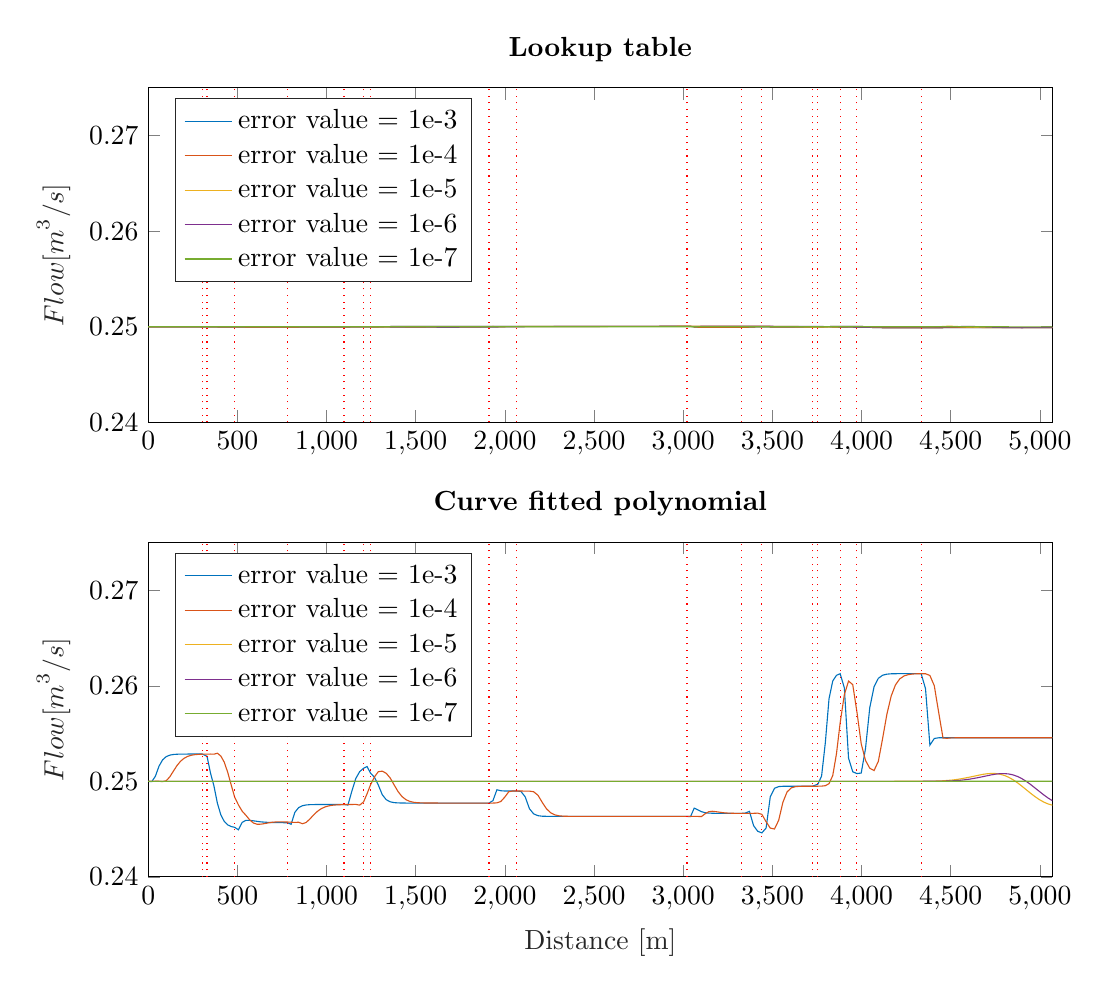
\begin{tikzpicture}

\begin{axis}[%
width=4.521in,
height=1.672in,
at={(0.758in,2.771in)},
scale only axis,
xmin=0,
xmax=5070,
xlabel style={font=\color{white!15!black}},
%xlabel={Distance [m]},
ymin=0.24,
ymax=0.275,
ylabel style={font=\color{white!15!black}},
ylabel={$\text{Flow [m}^\text{3}\text{/s]}$},
axis background/.style={fill=white},
title style={font=\bfseries},
title={Lookup table},
legend style={at={(0.03,0.97)}, anchor=north west, legend cell align=left, align=left, draw=white!15!black}
]
\addplot [color=mycolor1]
  table[row sep=crcr]{%
0	0.25\\
40.3999999999996	0.249995567863152\\
101	0.249978772543727\\
303	0.24997657629865\\
330	0.24997798809909\\
368.75	0.249985216471941\\
426.875	0.249961393024023\\
485	0.249956663435114\\
569.285714285715	0.249947860575958\\
716.785714285715	0.249939315043775\\
780	0.249939100412121\\
822.400000000001	0.249943103687656\\
886	0.249965594986861\\
1034.4	0.249970367805872\\
1098	0.249970385032611\\
1164	0.249982709545293\\
1208	0.249990038493706\\
1246	0.249980688303367\\
1268.16666666667	0.249970688922986\\
1290.33333333333	0.249975609645844\\
1334.66666666667	0.250014397078303\\
1401.16666666667	0.250023966850677\\
1911	0.250024452777325\\
2066	0.250032254170947\\
3021	0.25004626554346\\
3041.26666666667	0.250047344356062\\
3061.53333333333	0.249976124086061\\
3081.8	0.249950519231788\\
3122.33333333333	0.249938298209599\\
3325	0.249936628411888\\
3348.2	0.249938338079119\\
3417.8	0.249986721633832\\
3441	0.249989037648447\\
3488.16666666667	0.249975951472152\\
3535.33333333333	0.249959646902425\\
3724	0.249958843693094\\
3755	0.249958138675538\\
3775.83333333333	0.249959389843752\\
3838.33333333333	0.250035474116885\\
3880	0.25004106524284\\
3974	0.250034972771573\\
3998	0.25003390013444\\
4022	0.249996305934474\\
4046	0.249939924192404\\
4070	0.249911940360107\\
4118	0.249896863952927\\
4334	0.249894862917245\\
4824.66666666667	0.249908105777649\\
5070	0.249908105777649\\
};
\addlegendentry{error value = 1e-3}

\addplot [color=mycolor2]
  table[row sep=crcr]{%
0	0.25\\
40.3999999999996	0.249995567863152\\
101	0.249978772543727\\
303	0.24997657629865\\
330	0.24997798809909\\
368.75	0.249985216471941\\
426.875	0.249961393024023\\
485	0.249956663435114\\
569.285714285715	0.249947860575958\\
716.785714285715	0.249939315043775\\
780	0.249939100412121\\
822.400000000001	0.249943103687656\\
886	0.249965594986861\\
1034.4	0.249970367805872\\
1098	0.249970385032611\\
1164	0.249982709545293\\
1208	0.249990038493706\\
1246	0.249980688303367\\
1268.16666666667	0.249970688922986\\
1290.33333333333	0.249975609645844\\
1334.66666666667	0.250014397078303\\
1401.16666666667	0.250023966850677\\
1911	0.250024452777325\\
2066	0.250032254170947\\
3021	0.25004626554346\\
3041.26666666667	0.250047344356062\\
3061.53333333333	0.249976124086061\\
3081.8	0.249950519231788\\
3122.33333333333	0.249938298209599\\
3325	0.249936628411888\\
3348.2	0.249938338079119\\
3417.8	0.249986721633832\\
3441	0.249989037648447\\
3488.16666666667	0.249975951472152\\
3535.33333333333	0.249959646902425\\
3724	0.249958843693094\\
3755	0.249958138675538\\
3775.83333333333	0.249959389843752\\
3838.33333333333	0.250035474116885\\
3880	0.25004106524284\\
3974	0.250034972771573\\
3998	0.25003390013444\\
4022	0.249996305934474\\
4046	0.249939924192404\\
4070	0.249911940360107\\
4118	0.249896863952927\\
4334	0.249894862917245\\
4824.66666666667	0.249908105777649\\
5070	0.249908105777649\\
};
\addlegendentry{error value = 1e-4}

\addplot [color=mycolor3]
  table[row sep=crcr]{%
0	0.25\\
303	0.25\\
330	0.25\\
485	0.250000000020009\\
780	0.249999871538421\\
1034.4	0.249985380125509\\
1098	0.249981277749612\\
1208	0.249978170671056\\
1246	0.249977071332978\\
1401.16666666667	0.249961828437335\\
1489.83333333333	0.249936215392154\\
1578.5	0.24995517690877\\
1689.33333333333	0.249964538518725\\
1911	0.24997972248002\\
1933.14285714286	0.250027998627047\\
1955.28571428571	0.249990805581547\\
2066	0.250017724233658\\
2471.875	0.250024927235245\\
3021	0.25004609917778\\
3325	0.250046265189667\\
3441	0.250046265524361\\
3606.08333333333	0.250038446109102\\
3676.83333333333	0.250002768261766\\
3724	0.249972055863509\\
3755	0.249964642727718\\
3880	0.249942726602058\\
3974	0.249960301402098\\
4166	0.249965989329212\\
4334	0.249960956805808\\
4407.6	0.249976639430315\\
4456.66666666667	0.250023312768462\\
4481.2	0.250050367457334\\
4505.73333333333	0.250048976571634\\
4579.33333333333	0.249981248505719\\
4677.46666666667	0.249922143906588\\
4726.53333333333	0.249901781510744\\
4824.66666666667	0.249899058127085\\
5070	0.249908110746219\\
};
\addlegendentry{error value = 1e-5}

\addplot [color=mycolor4]
  table[row sep=crcr]{%
0	0.25\\
303	0.25\\
330	0.25\\
485	0.25\\
780	0.249999997836312\\
1098	0.249995392749042\\
1208	0.249986996849657\\
1246	0.249984342101925\\
1534.16666666667	0.249964151538734\\
1667.16666666667	0.249942420758998\\
1911	0.249967744211062\\
1999.57142857143	0.249982642687428\\
2043.85714285714	0.250002569626304\\
2066	0.249997764401087\\
2185.375	0.250011211507626\\
2352.5	0.250023742672056\\
3021	0.250043244100198\\
3325	0.25004624716621\\
3441	0.250046263997319\\
3724	0.250036205172364\\
3755	0.250030627799788\\
3817.5	0.250005613683243\\
3880	0.249971012010974\\
3974	0.249944980550026\\
4118	0.249955394117023\\
4262	0.249968167406223\\
4334	0.249965341594361\\
4481.2	0.249968489175444\\
4530.26666666667	0.249995113533259\\
4579.33333333333	0.2500359021642\\
4603.86666666667	0.250040179595999\\
4652.93333333333	0.250006360254702\\
4726.53333333333	0.249953187730171\\
4824.66666666667	0.24990486761908\\
4898.26666666667	0.249897701658483\\
5070	0.24990792891731\\
};
\addlegendentry{error value = 1e-6}

\addplot [color=mycolor5]
  table[row sep=crcr]{%
0	0.25\\
303	0.25\\
330	0.25\\
485	0.25\\
780	0.25\\
1098	0.25\\
1208	0.25\\
1246	0.25\\
1911	0.25\\
2066	0.25\\
3021	0.25\\
3325	0.25\\
3441	0.25\\
3724	0.25\\
3755	0.25\\
3880	0.25\\
3974	0.25\\
4334	0.25\\
5070	0.249987499462804\\
};
\addlegendentry{error value = 1e-7}

\addplot [color=red, dotted, forget plot]
  table[row sep=crcr]{%
303	0.240000000000009\\
303	0.274999999999977\\
};
\addplot [color=red, dotted, forget plot]
  table[row sep=crcr]{%
330	0.240000000000009\\
330	0.274999999999977\\
};
\addplot [color=red, dotted, forget plot]
  table[row sep=crcr]{%
485	0.240000000000009\\
485	0.274999999999977\\
};
\addplot [color=red, dotted, forget plot]
  table[row sep=crcr]{%
780	0.240000000000009\\
780	0.274999999999977\\
};
\addplot [color=red, dotted, forget plot]
  table[row sep=crcr]{%
1098	0.240000000000009\\
1098	0.275000000000091\\
};
\addplot [color=red, dotted, forget plot]
  table[row sep=crcr]{%
1208	0.240000000000009\\
1208	0.275000000000091\\
};
\addplot [color=red, dotted, forget plot]
  table[row sep=crcr]{%
1246	0.240000000000009\\
1246	0.275000000000091\\
};
\addplot [color=red, dotted, forget plot]
  table[row sep=crcr]{%
1911	0.240000000000009\\
1911	0.275000000000091\\
};
\addplot [color=red, dotted, forget plot]
  table[row sep=crcr]{%
2066	0.239999999999782\\
2066	0.275000000000091\\
};
\addplot [color=red, dotted, forget plot]
  table[row sep=crcr]{%
3021	0.239999999999782\\
3021	0.275000000000091\\
};
\addplot [color=red, dotted, forget plot]
  table[row sep=crcr]{%
3325	0.239999999999782\\
3325	0.275000000000091\\
};
\addplot [color=red, dotted, forget plot]
  table[row sep=crcr]{%
3441	0.239999999999782\\
3441	0.275000000000091\\
};
\addplot [color=red, dotted, forget plot]
  table[row sep=crcr]{%
3724	0.239999999999782\\
3724	0.275000000000091\\
};
\addplot [color=red, dotted, forget plot]
  table[row sep=crcr]{%
3755	0.239999999999782\\
3755	0.275000000000091\\
};
\addplot [color=red, dotted, forget plot]
  table[row sep=crcr]{%
3880	0.239999999999782\\
3880	0.275000000000091\\
};
\addplot [color=red, dotted, forget plot]
  table[row sep=crcr]{%
3974	0.239999999999782\\
3974	0.275000000000091\\
};
\addplot [color=red, dotted, forget plot]
  table[row sep=crcr]{%
4334	0.239999999999782\\
4334	0.274999999999636\\
};
\end{axis}

\begin{axis}[%
width=4.521in,
height=1.672in,
at={(0.758in,0.498in)},
scale only axis,
xmin=0,
xmax=5070,
xlabel style={font=\color{white!15!black}},
xlabel={Distance [m]},
ymin=0.24,
ymax=0.275,
ylabel style={font=\color{white!15!black}},
ylabel={$\text{Flow [m}^\text{3}\text{/s]}$},
axis background/.style={fill=white},
title style={font=\bfseries},
title={Curve fitted polynomial},
legend style={at={(0.03,0.97)}, anchor=north west, legend cell align=left, align=left, draw=white!15!black}
]
\addplot [color=mycolor1]
  table[row sep=crcr]{%
0	0.25\\
20.1999999999998	0.249963650951031\\
40.3999999999996	0.250538196492926\\
60.6000000000004	0.25158301884403\\
80.8000000000002	0.252246890232527\\
101	0.252585047782304\\
121.2	0.252740982194155\\
141.4	0.252808901929711\\
161.6	0.252837410399479\\
202	0.252853754484931\\
303	0.252856753405467\\
330	0.252616416962155\\
349.375	0.250862274120664\\
368.75	0.249512990073526\\
388.125	0.247705509939806\\
407.5	0.24647986106811\\
426.875	0.245791523068874\\
446.25	0.245438309827477\\
465.625	0.245266414948674\\
485	0.245185622263307\\
506.071428571428	0.244923374567406\\
527.142857142857	0.245707940899592\\
548.214285714286	0.245916990355909\\
569.285714285715	0.245918942281605\\
632.5	0.245754925254005\\
674.642857142857	0.245699070214869\\
716.785714285715	0.245676275665573\\
780	0.245666088077996\\
801.2	0.245503647709484\\
822.400000000001	0.246752404998915\\
843.6	0.24724966750091\\
864.8	0.247447777456728\\
886	0.247526690409359\\
907.2	0.247558103206757\\
949.6	0.247575579288423\\
1098	0.247578851827711\\
1120	0.247513515843821\\
1142	0.248970620217733\\
1164	0.250292250978418\\
1186	0.251022343734803\\
1208	0.251366375956422\\
1227	0.251551833500343\\
1246	0.25088009711817\\
1268.16666666667	0.250434294592196\\
1290.33333333333	0.249611533484313\\
1312.5	0.248601471891561\\
1334.66666666667	0.248076781978853\\
1356.83333333333	0.24785529671135\\
1379	0.247770350354585\\
1401.16666666667	0.247739525318138\\
1445.5	0.247725053954127\\
1711.5	0.247723218174542\\
1911	0.247723218172723\\
1933.14285714286	0.247979739018774\\
1955.28571428571	0.249117526988812\\
1977.42857142857	0.249012174816926\\
1999.57142857143	0.24898618790121\\
2066	0.248982065937525\\
2089.875	0.24894730055621\\
2113.75	0.248383160509547\\
2137.625	0.247136166959535\\
2161.5	0.246589840679007\\
2185.375	0.246404318915665\\
2209.25	0.246347850141319\\
2257	0.246327230953284\\
2543.5	0.24632560664395\\
3021	0.246325606637583\\
3041.26666666667	0.246314162984163\\
3061.53333333333	0.247195018164348\\
3081.8	0.247019533735511\\
3102.06666666667	0.246824380335056\\
3122.33333333333	0.246719760890301\\
3142.6	0.246673512801863\\
3183.13333333333	0.246647705551368\\
3304.73333333333	0.246643612004846\\
3325	0.246643603666598\\
3348.2	0.246681260416153\\
3371.4	0.246853370852477\\
3394.6	0.245356622147483\\
3417.8	0.24477161753839\\
3441	0.244601999392216\\
3464.58333333333	0.245106570498137\\
3488.16666666667	0.24838667104359\\
3511.75	0.249270684179464\\
3535.33333333333	0.249448895032401\\
3558.91666666667	0.249480818926713\\
3629.66666666667	0.249487148478693\\
3724	0.249487201772354\\
3755	0.249699562951719\\
3775.83333333333	0.250554853474569\\
3796.66666666667	0.254011602553874\\
3817.5	0.258642674254588\\
3838.33333333333	0.260498199752874\\
3859.16666666667	0.261091595200924\\
3880	0.261263185589996\\
3903.5	0.259774170101082\\
3927	0.252423556895337\\
3950.5	0.251000292119897\\
3974	0.250814026684566\\
3998	0.250864001387527\\
4022	0.253415764408601\\
4046	0.257709521211837\\
4070	0.259893949630168\\
4094	0.260779885336888\\
4118	0.261104788577541\\
4142	0.261217273423426\\
4166	0.261254781227763\\
4214	0.261270823014456\\
4334	0.261272586688392\\
4358.53333333333	0.259700070398139\\
4383.06666666667	0.253790141850914\\
4407.6	0.254484175186917\\
4432.13333333333	0.254556103392133\\
4505.73333333333	0.254561422759252\\
5070	0.254561444401588\\
};
\addlegendentry{error value = 1e-3}

\addplot [color=mycolor2]
  table[row sep=crcr]{%
0	0.25\\
60.6000000000004	0.250003468704563\\
80.8000000000002	0.24996681745597\\
101	0.250057830987316\\
121.2	0.250471159197332\\
141.4	0.251068576721082\\
161.6	0.251650758217693\\
181.8	0.252108526683514\\
202	0.252422241663226\\
222.2	0.252617481574816\\
242.4	0.252730591847467\\
262.6	0.252792583763949\\
282.8	0.252825090518854\\
303	0.252841533131686\\
330	0.252851964777619\\
349.375	0.252854426254089\\
368.75	0.252842663699994\\
388.125	0.252939723860436\\
407.5	0.252641552431669\\
426.875	0.251992073422116\\
446.25	0.250919101556974\\
465.625	0.249610037132697\\
485	0.248334646676994\\
506.071428571428	0.247531138021259\\
527.142857142857	0.246872266990067\\
548.214285714286	0.246440896563399\\
569.285714285715	0.245961960467866\\
590.357142857143	0.245634309794696\\
611.428571428572	0.245505633367429\\
632.5	0.245514941159854\\
695.714285714286	0.245716429336426\\
716.785714285715	0.245747627026503\\
737.857142857143	0.245757632951609\\
780	0.245741750726665\\
822.400000000001	0.245700405592288\\
843.6	0.245717858958415\\
864.8	0.245564274114258\\
886	0.245697384547384\\
907.2	0.24606893114742\\
928.400000000001	0.246498749505918\\
949.6	0.246869158795562\\
970.8	0.247141480025675\\
992	0.247322352362062\\
1013.2	0.247434237946436\\
1034.4	0.247499883034834\\
1055.6	0.247536851249606\\
1098	0.247567699446336\\
1164	0.247583032392868\\
1186	0.247508138761987\\
1208	0.247855479406098\\
1227	0.248685059190393\\
1246	0.249600916992677\\
1268.16666666667	0.250449520292022\\
1290.33333333333	0.25100697452217\\
1312.5	0.251063251890628\\
1334.66666666667	0.250839596811602\\
1356.83333333333	0.250351852628228\\
1379	0.249627573269208\\
1401.16666666667	0.248924886658642\\
1423.33333333333	0.248402538663868\\
1445.5	0.24807576668627\\
1467.66666666667	0.247894307209208\\
1489.83333333333	0.24780191802256\\
1512	0.247757878499215\\
1556.33333333333	0.2477292886133\\
1667.16666666667	0.247723270523238\\
1911	0.247723218173633\\
1933.14285714286	0.24772439597109\\
1955.28571428571	0.247745837034017\\
1977.42857142857	0.247893089901481\\
1999.57142857143	0.248349438098558\\
2021.71428571429	0.248910072662511\\
2043.85714285714	0.248990565781241\\
2066	0.248987261938055\\
2137.625	0.248975552412048\\
2161.5	0.248905260329593\\
2185.375	0.248546064243783\\
2209.25	0.247803972049951\\
2233.125	0.24712941978396\\
2257	0.246703688289017\\
2280.875	0.246485671355913\\
2304.75	0.246388227908028\\
2328.625	0.246348657103226\\
2376.375	0.246328337871091\\
2567.375	0.246325608026382\\
3021	0.246325606637583\\
3081.8	0.246325896004237\\
3102.06666666667	0.246310799265302\\
3122.33333333333	0.246597463305989\\
3142.6	0.246812878639503\\
3162.86666666667	0.246865566061388\\
3183.13333333333	0.246825860383069\\
3223.66666666667	0.246713956444182\\
3243.93333333333	0.246681053270549\\
3284.46666666667	0.24665244526841\\
3325	0.246645368682039\\
3394.6	0.246651237100195\\
3417.8	0.246669463091166\\
3441	0.246542642534223\\
3464.58333333333	0.245772902900171\\
3488.16666666667	0.245105168564805\\
3511.75	0.245007180378707\\
3535.33333333333	0.245925987143892\\
3558.91666666667	0.247805581513603\\
3582.5	0.248897479922562\\
3606.08333333333	0.249315364984795\\
3629.66666666667	0.249443069610606\\
3653.25	0.249476847778169\\
3700.41666666667	0.249486703152797\\
3724	0.249487069815586\\
3755	0.249489372113203\\
3775.83333333333	0.249498199676054\\
3796.66666666667	0.249542685759479\\
3817.5	0.249755129942969\\
3838.33333333333	0.25059906959541\\
3859.16666666667	0.25287238232886\\
3880	0.256126956573098\\
3903.5	0.259075873055735\\
3927	0.26049251706263\\
3950.5	0.26012255371279\\
3974	0.257258638476742\\
3998	0.253934947740163\\
4022	0.252188210348322\\
4046	0.251372475279823\\
4070	0.25112773364981\\
4094	0.252090888303428\\
4118	0.254482685211769\\
4142	0.257022432263511\\
4166	0.258923670156037\\
4190	0.26009054032329\\
4214	0.260719249368776\\
4238	0.261027963895685\\
4262	0.261169312267157\\
4286	0.261230600699491\\
4310	0.26125605314337\\
4334	0.261266240799159\\
4358.53333333333	0.261259864668318\\
4383.06666666667	0.26108076825949\\
4407.6	0.260018647038123\\
4432.13333333333	0.257242006845445\\
4456.66666666667	0.254525439539066\\
4481.2	0.254505921921918\\
4505.73333333333	0.254552158010483\\
4554.8	0.254561288847981\\
5070	0.254561444401588\\
};
\addlegendentry{error value = 1e-4}

\addplot [color=mycolor3]
  table[row sep=crcr]{%
0	0.25\\
303	0.25\\
330	0.25\\
485	0.25\\
780	0.25\\
1098	0.25\\
1208	0.25\\
1246	0.25\\
1911	0.25\\
2066	0.25\\
3021	0.25\\
3325	0.25\\
3441	0.25\\
3724	0.25\\
3755	0.25\\
3880	0.250000000020009\\
3974	0.250000001361514\\
4334	0.250003638736416\\
4407.6	0.250021244655727\\
4456.66666666667	0.250056621295698\\
4505.73333333333	0.250128930993014\\
4530.26666666667	0.250183963570635\\
4554.8	0.250253019240517\\
4603.86666666667	0.25042972481333\\
4677.46666666667	0.250721155392057\\
4702	0.250790467678598\\
4726.53333333333	0.25082621537058\\
4751.06666666667	0.250816046942418\\
4775.6	0.250749675285988\\
4800.13333333333	0.25062011533646\\
4824.66666666667	0.250424815728366\\
4849.2	0.250166754280144\\
4873.73333333333	0.249854848681935\\
4898.26666666667	0.249503451044802\\
4947.33333333333	0.248758221366188\\
4971.86666666667	0.248405720639312\\
4996.4	0.248092062929572\\
5020.93333333333	0.247831946980114\\
5045.46666666667	0.2476350413408\\
5070	0.247505838177858\\
};
\addlegendentry{error value = 1e-5}

\addplot [color=mycolor4]
  table[row sep=crcr]{%
0	0.25\\
303	0.25\\
330	0.25\\
485	0.25\\
780	0.25\\
1098	0.25\\
1208	0.25\\
1246	0.25\\
1911	0.25\\
2066	0.25\\
3021	0.25\\
3325	0.25\\
3441	0.25\\
3724	0.25\\
3755	0.25\\
3880	0.250000000000909\\
3974	0.25000000010823\\
4334	0.250000717624971\\
4456.66666666667	0.250017552722966\\
4505.73333333333	0.25004750347307\\
4554.8	0.250110132776172\\
4603.86666666667	0.250220753277972\\
4652.93333333333	0.250383753941605\\
4726.53333333333	0.250672150635182\\
4751.06666666667	0.25074991285237\\
4775.6	0.250800427911599\\
4800.13333333333	0.250811425660686\\
4824.66666666667	0.250771929666371\\
4849.2	0.250673538856972\\
4873.73333333333	0.250511604824169\\
4898.26666666667	0.25028641278368\\
4922.8	0.250003750110409\\
4947.33333333333	0.249675077094253\\
5020.93333333333	0.248587837282685\\
5045.46666666667	0.248257418708818\\
5070	0.247972495508293\\
};
\addlegendentry{error value = 1e-6}

\addplot [color=mycolor5]
  table[row sep=crcr]{%
0	0.25\\
303	0.25\\
330	0.25\\
485	0.25\\
780	0.25\\
1098	0.25\\
1208	0.25\\
1246	0.25\\
1911	0.25\\
2066	0.25\\
3021	0.25\\
3325	0.25\\
3441	0.25\\
3724	0.25\\
3755	0.25\\
3880	0.25\\
3974	0.25\\
4334	0.25\\
5045.46666666667	0.250009617695468\\
5070	0.25001573595091\\
};
\addlegendentry{error value = 1e-7}

\addplot [color=red, dotted, forget plot]
  table[row sep=crcr]{%
303	0.240000000000009\\
303	0.274999999999977\\
};
\addplot [color=red, dotted, forget plot]
  table[row sep=crcr]{%
330	0.240000000000009\\
330	0.274999999999977\\
};
\addplot [color=red, dotted, forget plot]
  table[row sep=crcr]{%
485	0.240000000000009\\
485	0.274999999999977\\
};
\addplot [color=red, dotted, forget plot]
  table[row sep=crcr]{%
780	0.240000000000009\\
780	0.274999999999977\\
};
\addplot [color=red, dotted, forget plot]
  table[row sep=crcr]{%
1098	0.240000000000009\\
1098	0.275000000000091\\
};
\addplot [color=red, dotted, forget plot]
  table[row sep=crcr]{%
1208	0.240000000000009\\
1208	0.275000000000091\\
};
\addplot [color=red, dotted, forget plot]
  table[row sep=crcr]{%
1246	0.240000000000009\\
1246	0.275000000000091\\
};
\addplot [color=red, dotted, forget plot]
  table[row sep=crcr]{%
1911	0.240000000000009\\
1911	0.275000000000091\\
};
\addplot [color=red, dotted, forget plot]
  table[row sep=crcr]{%
2066	0.239999999999782\\
2066	0.275000000000091\\
};
\addplot [color=red, dotted, forget plot]
  table[row sep=crcr]{%
3021	0.239999999999782\\
3021	0.275000000000091\\
};
\addplot [color=red, dotted, forget plot]
  table[row sep=crcr]{%
3325	0.239999999999782\\
3325	0.275000000000091\\
};
\addplot [color=red, dotted, forget plot]
  table[row sep=crcr]{%
3441	0.239999999999782\\
3441	0.275000000000091\\
};
\addplot [color=red, dotted, forget plot]
  table[row sep=crcr]{%
3724	0.239999999999782\\
3724	0.275000000000091\\
};
\addplot [color=red, dotted, forget plot]
  table[row sep=crcr]{%
3755	0.239999999999782\\
3755	0.275000000000091\\
};
\addplot [color=red, dotted, forget plot]
  table[row sep=crcr]{%
3880	0.239999999999782\\
3880	0.275000000000091\\
};
\addplot [color=red, dotted, forget plot]
  table[row sep=crcr]{%
3974	0.239999999999782\\
3974	0.275000000000091\\
};
\addplot [color=red, dotted, forget plot]
  table[row sep=crcr]{%
4334	0.239999999999782\\
4334	0.274999999999636\\
};
\end{axis}
\end{tikzpicture}%
\caption{Various values of error value are tested with the lookup table and curve fitted polynomial tested on pipe setup shown in figure \ref{fig:Fredericia_pipe_setup} of Fredericia.}
\label{fig:error_value_test}
\end{figure} 

If the curve fitted polynomial is utilized to obtain boundary conditions then an error value below $1\cdot10^{-6}$ is preferable. But for setup's with more pipes, it can be necessary to lower this value even further. The lookup table, on the other hand, is due to its better precision not considerably affected in the first place, though some precision is obtained by lowering the error value. As the tested error value is performed on a simple test, and a final decision has not been made on which scheme to utilize an error value of $1\cdot10^{-9}$ has been decided upon. The reason being the results shown in figure \ref{fig:error_value_test}, and that various setup where more pipes with different initial flows might yield a worse result.

\subsection*{Simulation}

Having obtained initial data, for which iterating with the Preissmann scheme can begin, the next part to be implemented is the simulation of the initialized setup.
To ease eventual future expansion of the simulation a simple design, where individual parts are simulated one at a time, is chosen. This is realized by nesting functions in two steps from the main simulation module which is seen in figure \ref{fig:simu_main_chart}.

\begin{figure}[H]
\centering
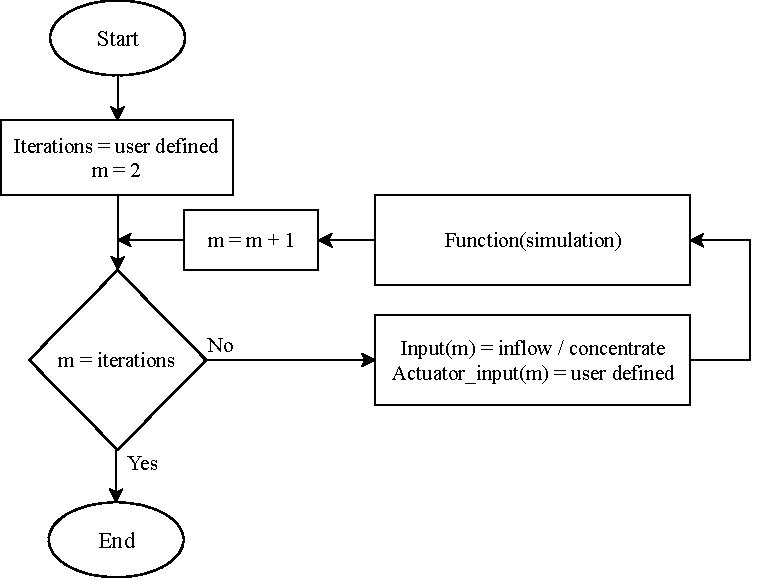
\includegraphics[width=0.7 \textwidth]{report/simulation/pictures/simu_main_chart.pdf}
\caption{Main simulation loop.}
\label{fig:simu_main_chart}
\end{figure}

The number of iterations desired to simulate the system for is chosen. As the system is already initialized and MATLAB does not have zero indexing the system is initialized at m equal to one. Therefore the first iteration is performed at m equal to two and proceeds until the chosen amount of iterations is reached. The function ``simulation'' is given flow and concentrate input, system specification (Sys\_setup), pipe specification (pipe\_spec). If a tank is present, actuator input and tank specification (tank\_spec) are also needed.
In figure \ref{fig:simu_chart} the simulation function is seen.
\begin{figure}[H]
\centering
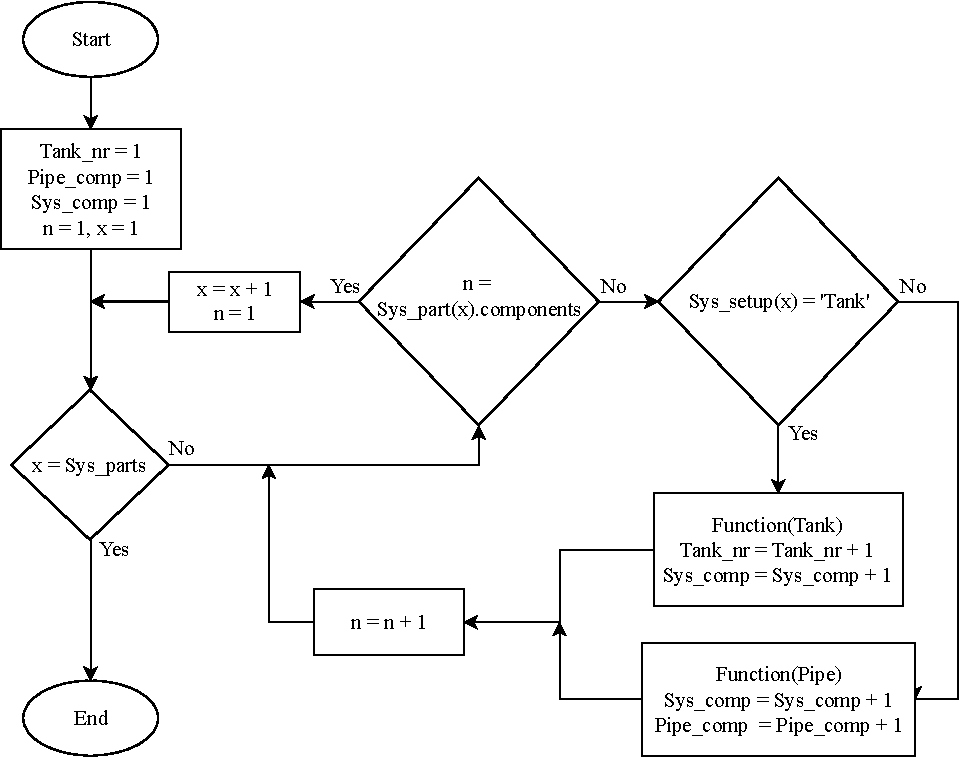
\includegraphics[width=0.9 \textwidth]{report/simulation/pictures/simu_chart.pdf}
\caption{Simulation function.}
\label{fig:simu_chart}
\end{figure}

The simulation function is given input of flow, concentrate and actuator for pipes and tanks respectively. Furthermore specifications of system, pipe and tank are given. The basic functionality is an outer and an inner loop. The outer loop iterates through the parts in ``Sys\_setup'' and the inner loop iterates through the components each part consists of. Iterating through the parts, checking whether the component is a tank or pipe, the respective function is called. The tank function is given tank specifications, current iteration value, flow and actuator input. Furthermore, the index number of the tank is given. The iteration value ``m'' is in the function used to index when logging data. Output flow is found by equation \ref{eq:control_signal_pump_tank}. The value of $\overline Q$ in equation \ref{eq:control_signal_pump_tank} is set to be the maximum inflow of the adjoining pipe as seen below. 
\begin{equation}\label{eq:imp_tank_outflow}
	Q_{out} = u_{pump} \cdot Q_{max\_outflow}
\end{equation} 
Where maximum outflow is equal to the maximum inflow of the downstream adjoining pipe.
Doing so makes it possible to always have an actuator input which ranges from zero to one, which helps to minimize complexity when implementing control on large scale setups where several tanks of various sizes could be present. In figure \ref{fig:tank_function} a flow chart of the tank function can be seen.

\begin{figure}[H]
\centering
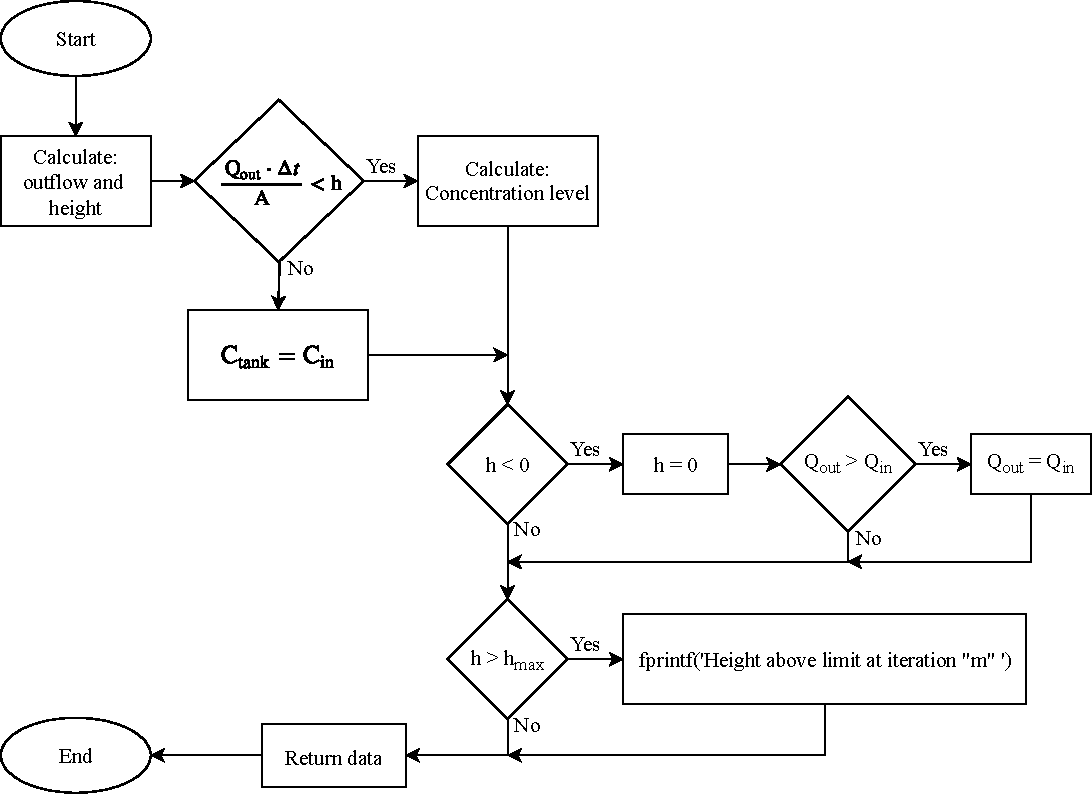
\includegraphics[width=0.95 \textwidth]{report/simulation/pictures/tank_function.pdf}
\caption{Tank function.}
\label{fig:tank_function}
\end{figure}

The tank function is given inflow, actuator input, ``Tank\_nr'', tank specification, iteration value ``m'', part index ``x'' and data stored at index ``Sys\_comp''. Iteration and part index is used to fetch previous values of height and concentrate level, used in the calculation of new values. Furthermore the value of ``Tank\_nr'' is used as index in ``Tank\_spec''.
First, when the height and flow has been calculated, the condition mentioned in section \ref{sec:tank} is checked to avoid oscillating concentrate level in the tank. %Secondly the considerations mentioned in section \ref{sec:tank} is needed when fluid height goes towards zero. 
Secondly, as seen in the flowchart, if the calculated height gives a result below zero the height is set to zero and maximum outflow is set equal to inflow. In the case of concentrate level, if height is less than $\text{Q}_\text{out} \cdot \Delta t / \text{A}$ then the level in the tank is set equal to the inflow level. If the fluid level exceeds the height of the tank a message is printed to the command windows which also contains at which iteration the overflow occurred. Instead of placing a hard limit on tank height, knowing when a tank overflow occurs, and how much the dimension of the tank needs to be adjusted, would be more valuable. 
In figure \ref{fig:pipe_function} the pipe function can be seen.

\begin{figure}[H]
\centering
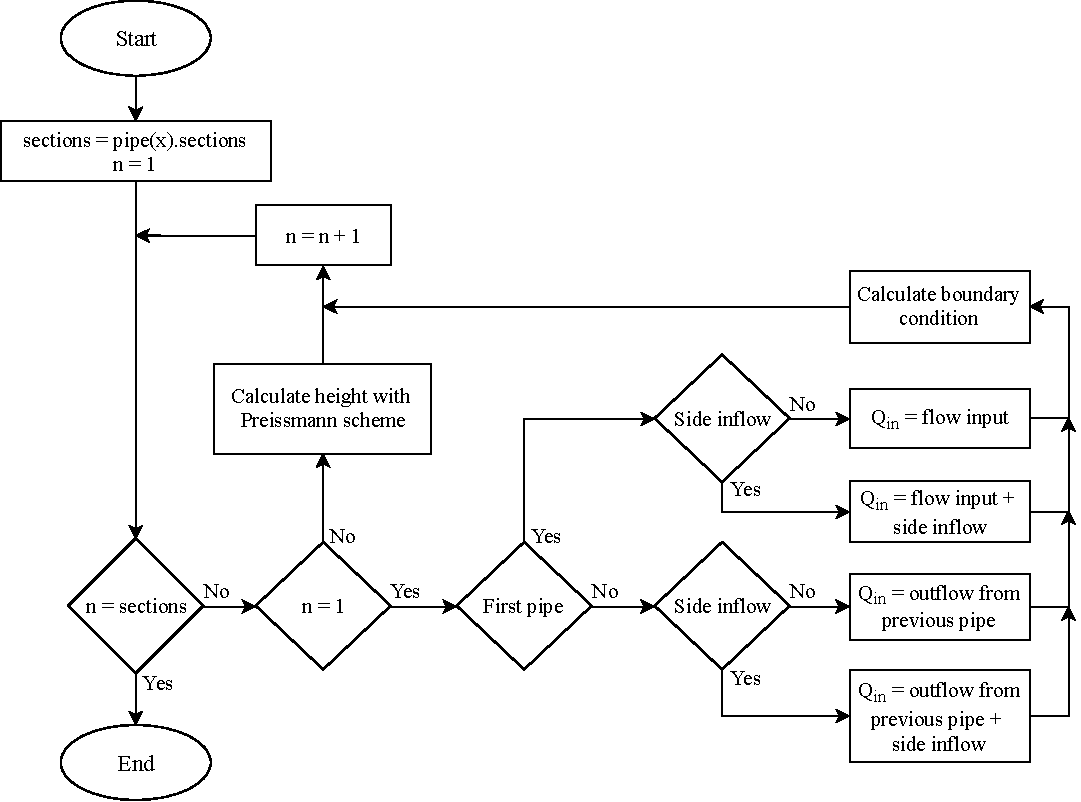
\includegraphics[width=0.9 \textwidth]{report/simulation/pictures/pipe_function.pdf}
\caption{Pipe function.}
\label{fig:pipe_function}
\end{figure}

The function is given inflow, pipe\_comp, pipe specifications, iteration value ``m'', part index ``x'' and data stored at index ``Sys\_comp''.
Once again iteration and part index are used to fetch previous values of height and concentrate level, used in the calculation of new values. The value of pipe\_comp is used as an index in ``pipe\_spec''. The functionality of the function is to iterate through the sections which the pipe consists of.
At the first section, n = 1, it is determined if the pipe is the first in the specific part. Afterward, it is checked if side inflow is present. If the pipe is the first then inflow needs to be given, otherwise the flow out of the previous pipe is set as inflow. When inflow is obtained, height can be found from either curve fitted polynomial or lookup table as mentioned in the initialization part of the implementation. For the remaining sections in the pipe, the height is found by the Preissmann scheme. Finally, data is returned to the simulation function.
To decided upon which of the curve fitted polynomial or lookup table, methods should be implemented a test with the pipe setup shown in figure \ref{fig:Fredericia_pipe_setup} is performed for various iterations. Furthermore, two values of $\Delta t$ are tested. A  sinusoidal input is given for all tests to increase the computational power needed to solve the Preissmann scheme. The input can be seen in figure \ref{fig:comparison_look_fit_input}.
\begin{figure}[H]
 \centering
 % This file was created by matlab2tikz.
%
%The latest updates can be retrieved from
%  http://www.mathworks.com/matlabcentral/fileexchange/22022-matlab2tikz-matlab2tikz
%where you can also make suggestions and rate matlab2tikz.
%
\definecolor{mycolor1}{rgb}{0.00000,0.44700,0.74100}%
%
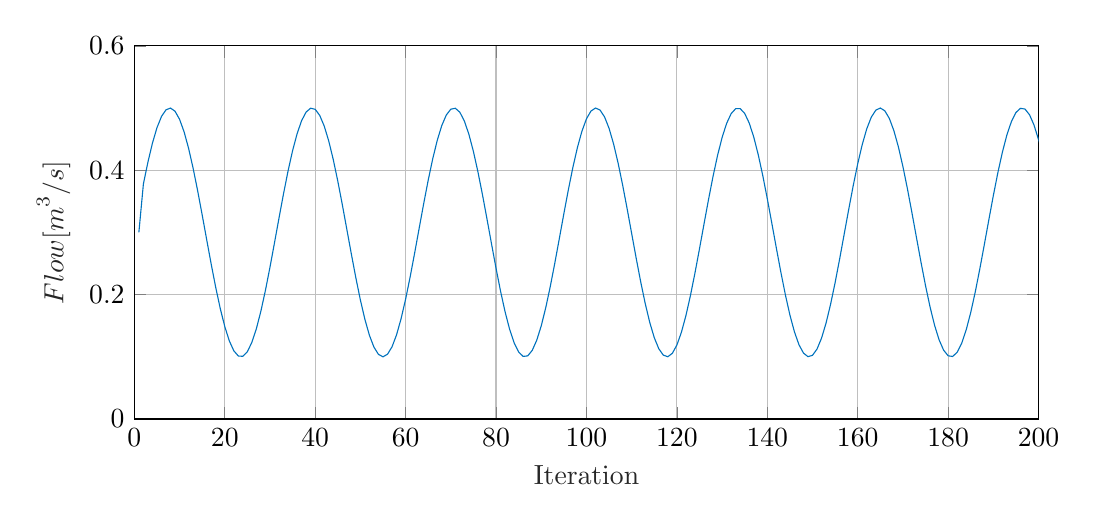
\begin{tikzpicture}

\begin{axis}[%
width=4.521in,
height=1.866in,
at={(0.758in,0.481in)},
scale only axis,
xmin=0,
xmax=200,
xlabel style={font=\color{white!15!black}},
xlabel={Iteration},
ymin=0,
ymax=0.6,
ylabel style={font=\color{white!15!black}},
ylabel={$\text{Flow [m}^\text{3}\text{/s]}$},
axis background/.style={fill=white},
xmajorgrids,
ymajorgrids,
legend style={legend cell align=left, align=left, draw=white!15!black}
]
\addplot [color=mycolor1]
  table[row sep=crcr]{%
1	0.300000000000011\\
2	0.37788366846172\\
3	0.412928494678994\\
4	0.443471218179894\\
5	0.46829419696158\\
6	0.486407817193452\\
7	0.497089945997686\\
8	0.499914720608302\\
9	0.494769526175645\\
10	0.481859485365135\\
11	0.461699280763924\\
12	0.435092636110227\\
13	0.403100274364306\\
14	0.366997630031193\\
15	0.328224001611972\\
16	0.288325171314483\\
17	0.248891779594629\\
18	0.211495911341018\\
19	0.177628421811448\\
20	0.148639500938401\\
21	0.12568484551727\\
22	0.109679585222096\\
23	0.101261799273317\\
24	0.10076707823282\\
25	0.108215145067362\\
26	0.123309068855974\\
27	0.145447102488816\\
28	0.173746672425523\\
29	0.207079564117237\\
30	0.244116900360211\\
31	0.28338211943651\\
32	0.323309840970097\\
33	0.362308272702677\\
34	0.39882267022773\\
35	0.431397319743752\\
36	0.45873357276983\\
37	0.479741619162326\\
38	0.493583934406303\\
39	0.49970866907492\\
40	0.497871649324679\\
41	0.488146111335965\\
42	0.470919781617653\\
43	0.446879419574827\\
44	0.416983438578342\\
45	0.382423697048353\\
46	0.344577982820056\\
48	0.265134643755403\\
49	0.226704174149603\\
50	0.191195777822116\\
51	0.160025062481282\\
52	0.134434706182873\\
53	0.115444915677443\\
54	0.103812753986688\\
55	0.100001958689859\\
56	0.104164454169734\\
57	0.116134294867067\\
58	0.135434281006269\\
59	0.16129498304457\\
60	0.192685416399911\\
61	0.228354143552622\\
62	0.266879164910335\\
63	0.306724609444217\\
64	0.346301965020302\\
65	0.384033407365337\\
66	0.418414702941448\\
67	0.448075177990489\\
68	0.471832362971298\\
69	0.488739133888828\\
70	0.498121471138973\\
71	0.499605330543261\\
72	0.493131555309844\\
73	0.478958234428092\\
74	0.457650413475051\\
75	0.43005756803143\\
76	0.397279737770759\\
77	0.360623671349146\\
78	0.321550730459876\\
79	0.281618629954465\\
80	0.242419336666984\\
81	0.205515602720311\\
82	0.172378663530424\\
83	0.144329584293132\\
84	0.122486593283696\\
85	0.107720501624101\\
86	0.100619986791685\\
87	0.101468123905875\\
88	0.110231100416371\\
89	0.126559564102877\\
90	0.14980255064566\\
91	0.179033435518733\\
92	0.213086875585617\\
93	0.250605267652674\\
94	0.290092871824328\\
95	0.329975441932589\\
96	0.36866298576399\\
97	0.404613153031534\\
98	0.436392724013615\\
99	0.462734747501429\\
100	0.482589050145521\\
101	0.495164103553407\\
102	0.499958580028533\\
103	0.496781338923711\\
104	0.485759046815446\\
105	0.467331127707212\\
106	0.442232244581191\\
107	0.411463010703528\\
108	0.376250098330985\\
109	0.337997335159088\\
111	0.258532715878658\\
112	0.220488863375721\\
113	0.185614868978092\\
114	0.155301048791159\\
115	0.130755919164955\\
116	0.112958016961102\\
117	0.102616888375877\\
118	0.100144801572668\\
119	0.105640310851214\\
120	0.118884327598664\\
121	0.139348854661222\\
122	0.166218035924402\\
123	0.198420681921874\\
124	0.234672974779045\\
125	0.273529649980446\\
126	0.313441614505109\\
127	0.352817704276902\\
128	0.39008811885509\\
129	0.423767004424008\\
130	0.452511690095918\\
131	0.475176215962165\\
132	0.490857018898538\\
133	0.498928954775579\\
134	0.499070220982304\\
135	0.491275185680905\\
136	0.475854612330153\\
137	0.453423270527111\\
138	0.424875427083265\\
139	0.391349194428841\\
140	0.354181157661571\\
141	0.314853089116866\\
142	0.274932874780717\\
143	0.236012007623174\\
144	0.199642139795884\\
145	0.167273223157395\\
146	0.140195704268081\\
147	0.119489078357958\\
148	0.105978853258563\\
149	0.100203639010601\\
150	0.102393675181418\\
151	0.112461651939952\\
152	0.130006190824133\\
153	0.154327846433688\\
154	0.184456991110864\\
155	0.219192470935383\\
156	0.257149491940822\\
158	0.336607145796108\\
159	0.374940052729897\\
160	0.410285336248336\\
161	0.44123389143607\\
162	0.466551897061549\\
163	0.485230004136099\\
164	0.496523575472821\\
165	0.499982372021464\\
166	0.495468502478445\\
167	0.483161920578169\\
168	0.463553250905278\\
169	0.437424229240946\\
170	0.405816537224013\\
171	0.369990273791331\\
172	0.33137371900969\\
173	0.291506393056608\\
174	0.251977680409254\\
175	0.214363466100764\\
176	0.180163310157155\\
177	0.150740664871023\\
178	0.127268518261417\\
179	0.110682630743014\\
180	0.101644229311376\\
181	0.100513646509285\\
182	0.107335955105242\\
183	0.121839171184632\\
184	0.143445097289856\\
185	0.171292373328612\\
186	0.204270816282303\\
187	0.241065679699943\\
188	0.280210068489936\\
189	0.320143419398505\\
190	0.359273715741864\\
191	0.39604095608766\\
192	0.42897934658896\\
193	0.456775737559667\\
194	0.478321974608292\\
195	0.492759077256807\\
196	0.499511483781561\\
197	0.498309997042838\\
198	0.489202516525381\\
199	0.472552128737135\\
200	0.449022632095875\\
201	0.419552073381055\\
};
%\addlegendentry{data1}

\end{axis}
\end{tikzpicture}%
\caption{Input flow for the comparison test of lookup table and curve fitted polynomial.}
\label{fig:comparison_look_fit_input}
\end{figure} 

The results of the computational tests can be seen in table \ref{400_it_comput}, \ref{800_it_comput} and \ref{2000_it_comput}.  

\begin{table}[H]
\centering
\begin{tabular}{|l|l|l|} \hline
	\rowcolor[HTML]{9B9B9B} 
			&  Run 1 & Run 2 \\ \hline
$\Delta t$ &	15 s & 20 s \\ \hline
lookup table &	4,600 s	&	4,978 s \\ \hline
Curve fitted  & \multirow{2}{*}{5,554 s} & \multirow{2}{*}{5,893 s} \\ 
polynomial    &						   &						\\ \hline
Difference    & 20.722 \%			   &  18.393 \% \\ \hline 
\end{tabular}
\caption{Computation time of 400 iterations.}
\label{400_it_comput}
\end{table}

\begin{table}[H]
\centering
\begin{tabular}{|l|l|l|} \hline
	\rowcolor[HTML]{9B9B9B} 
			&  Run 1 & Run 2 \\ \hline
$\Delta t$ 		&	15 s		& 	20 s \\ \hline
lookup table 	&	10,073 s	&	10,574 s \\ \hline
Curve fitted  	& \multirow{2}{*}{11,868 s} & \multirow{2}{*}{11,859 s} \\ 
polynomial    &						   &						\\ \hline
Difference    & 17.817 \%			   &  12.153 \% \\ \hline 
\end{tabular}
\caption{Computation time of 800 iterations.}
\label{800_it_comput}
\end{table}

\begin{table}[H]
\centering
\begin{tabular}{|l|l|l|} \hline
	\rowcolor[HTML]{9B9B9B} 
			&  Run 1 & Run 2 \\ \hline
$\Delta t$ 		&	15 s		& 	20 s \\ \hline
lookup table 	&	30,380 s	&	30,776 s  \\ \hline
Curve fitted 	& \multirow{2}{*}{33,247 s} & \multirow{2}{*}{34,194 s} \\ 
polynomial    	&						   &						\\ \hline
Difference    	& 9.437 \%			   &  11.105 \% \\ \hline 
\end{tabular}
\caption{Computation time of 2000 iterations.}
\label{2000_it_comput}
\end{table}

The results are obtained by using the MATLAB function ``tic-toc'' on the main simulation loop shown in figure \ref{fig:simu_main_chart}. Furthermore, a laptop with an I7-4710MQ processor at 3,4 GHz is used for the test. Clearly, the lookup table is preferable both in accuracy and computational speed. For this reason, it is implemented as the solution to obtain fluid height boundary condition from an inflow of the pipe.

\subsection*{Display result}

The areas of interest chosen to be displayed are, as mentioned in section \ref{sec:Structure}, flow, height, concentrate and concentrate flow.
In figure \ref{fig:data_plot_chart} a flowchart of the constructed playback function to examine the simulation result is seen 

\begin{figure}[H]
\centering
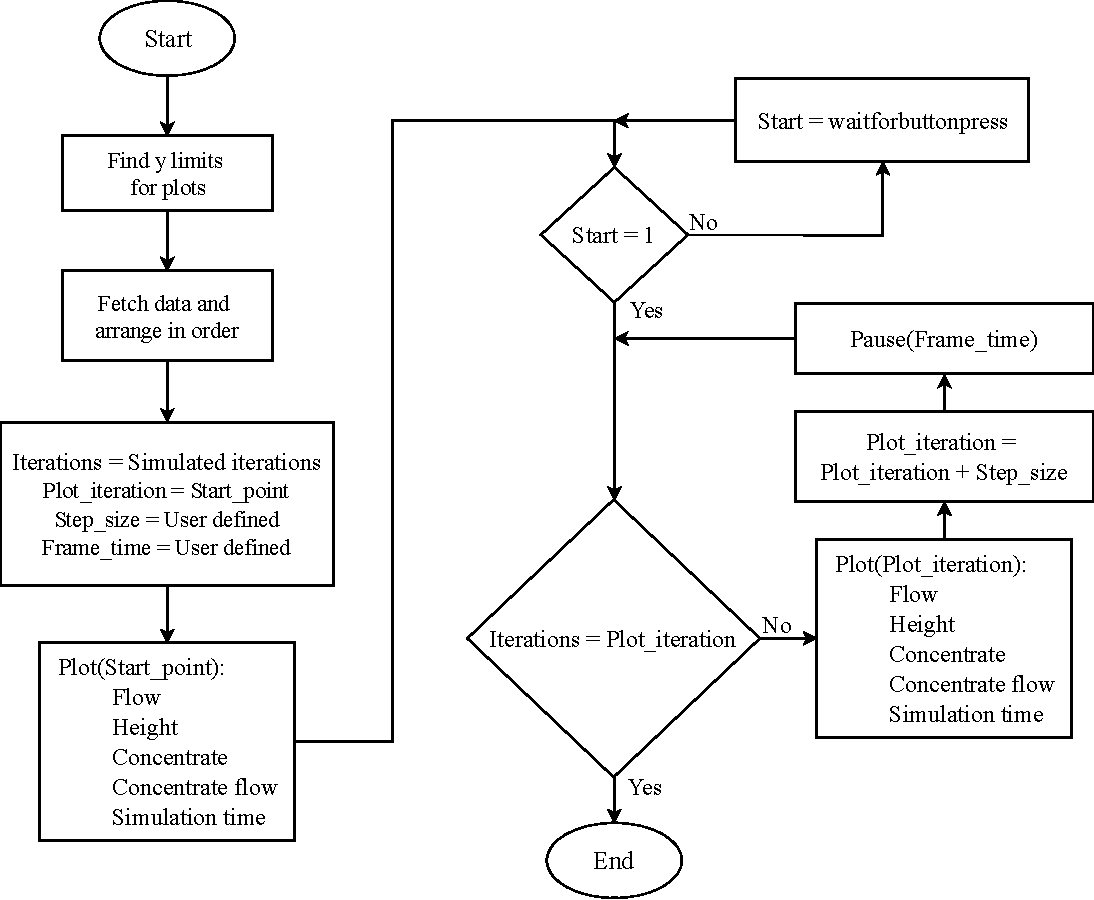
\includegraphics[width=0.9 \textwidth]{report/simulation/pictures/data_plot_chart.pdf}
\caption{Flowchart of playback function.}
\label{fig:data_plot_chart}
\end{figure}

%The playback function is constructed such that firstly minimum and maximum values on the y axis is limited to the variations in the data. 
The first thing that is done in the playback function is finding minimum and maximum values for the y-axis. This is done such that the graph can not move outside the plot. Furthermore, another setting where space, corresponding to a user defined percentage, at the top and bottom of the plot is unused. An initial value of ten percent at top and bottom is set, which leaves 80 percent of the window to be used by the graph during playback.  
Secondly, the data for all the components are fetched into a matrix such that the MATLAB plot function can be utilized. Furthermore, x-axis data is scaled correctly according to the number of components, various $\Delta x$, intersections and tanks. Afterward ``Iteration'' is set to the value of iterations which has been simulated, ``Plot\_iteration'' is set to the iteration from where the playback is to start from, ``step\_size'' is set to the number of iterations to skip during playback. Lastly ``frame\_time'' is set, which decides the speed of the playback. The maximum speed is in the end decided by the processor available to MATLAB and due to the plot function is known to be computationally demanding, a low amount of updates per second should be expected. The defined iteration or boundary conditions, if ``Start\_point'' is set to zero, is plotted before the playback is put on hold. Playback is now started by clicking on the window holding the plots and continues iterating in the predefined step size and frame time.


 \begin{sidewaysfigure}
 \centering
 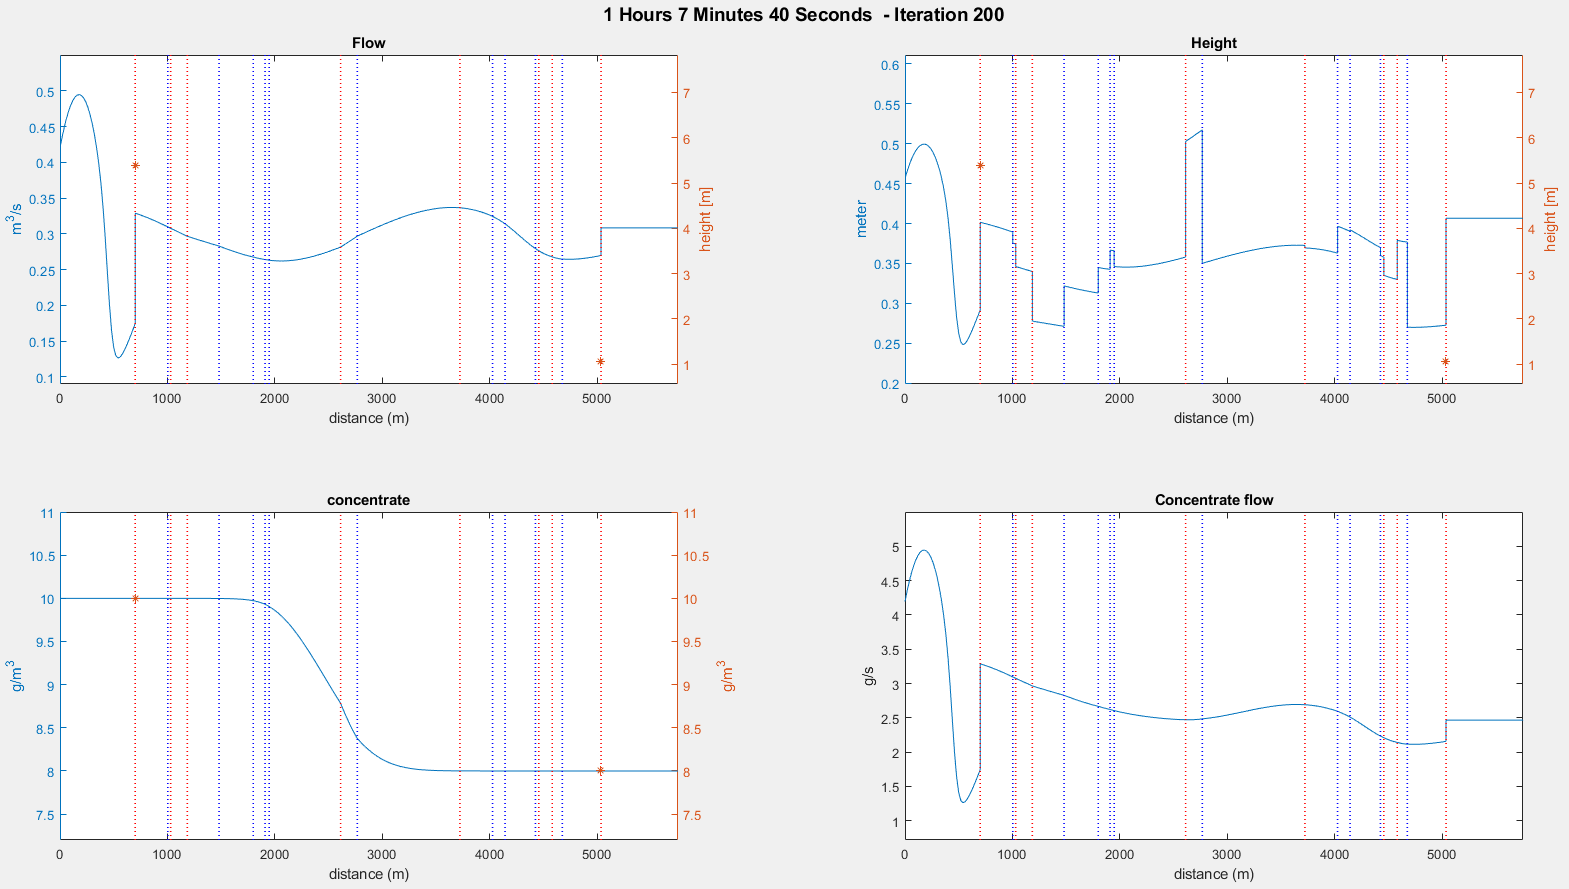
\includegraphics[width=1.0 \textwidth]{report/simulation/pictures/display_result_matlab.png}
 \caption{Screen shot of the plots made by the playback function where a sinusoidal flow input and step in concentrate is given, red dotted lines indicate pipe intersection and blue dotted lines are intersections with side inflow and stars are tanks inserted. In the simulation the pipe configuration seen in figure \ref{fig:Fredericia_pipe_setup} is used and input to the side inflows is not given.}
 \label{fig:display_result_matlab}
 \end{sidewaysfigure}
\fxnote{Sørg for at den her tykke figur vender rigtig i forhold til siden den er på}

This concludes on the implementation part of the simulation. The next section will go into details about the setup of the model predictive control scheme chosen for this project.